La biogéographie est l'étude de la répartition géographiques des
espèces. Aujourd'hui, ce terme est souvent remplacé par celui de
macroécologie. Outre la distinction historique, ce dernier terme met en
avant l'importance du raport des espèces à leur environnement plutôt que
la dimension évolutive (tout aussi importante). C'est pour garder à
l'esprit la richesse des facteurs qui dessinent les aires de répartition
que je garde le terme de biogéographie dont je dresse un portrait dans
la présente introduction. J'y abrode aussi bien la complexité de la
compréhension de la distribution spatiale des espèces que les cadres
théoriques actuels. Chemin faisant, je discute de l'importance du lien
qu'il existe entre les interactions écologiques et la répartition des
espèces ; cette réflexion est l'essence même de ma thèse.

\section*{Des îles et des espèces}\label{des-uxeeles-et-des-espuxe8ces}
\addcontentsline{toc}{section}{Des îles et des espèces}

\subsection*{En suivant Wallace}\label{en-suivant-wallace}
\addcontentsline{toc}{subsection}{En suivant Wallace}

Dans l'introduction de son livre \emph{Island Life} paru en 1881, le
célèbre naturaliste Alfred Russel Wallace nous rapporte deux faits
étonnants qui justifient pleinement l'examen attentif de la répartition
géographique des espèces (Wallace, 1881). Premièrement, le biogéographe
démontre, à l'aide de nombreux exemples, que l'éloignement entre deux
régions du monde n'est pas suffisant pour conclure quand à l'éloignement
de leur composition faunistique et floristique. Ainsi, la comparaison
des avifaunes du l'île japonnaise d'Hokkaido et de l'Angleterre,
séparées par des miliers de kilomètres, révèle une proximité des
paysages ornithologiques très supérieure à celle constatée quand on
compare les oiseaux des îles indonésiennes de Bali et de Lombok pourtant
distantes de seulement quelques kilomètres. Deuxièmement, en s'appuyant
sur les différences des faunes brésiliennes et africaines, Wallace
souligne la faiblesse du pouvoir prédictif des variables climatiques
pour décrire les compositions faunistiques présentes sous des latitudes
similaires. Ces constatations souligne l'utilité de croiser les
informations des distributions à la lumière d'une analyse taxonomique
pour y apporter du sens. Dans le cadre de la théorie de
l'évolution\footnote{Wallace a publié en 1858 un article \emph{On the
  Tendency of Varieties to Depart Indefinitely From the Original Type}
  qui témoigne très clairement que ses idées sur les varitions
  temporelles des espèces étaient très proche de celle de Charles Robert
  Darwin a qui il avait d'ailleurs envoyé le manuscipt (Wallace, 1858).},
encore toute jeune en 1881, cette analyse taxonomique est une analyse
historique : Wallace montre que la compréhension d'un problème spatial,
celui des aires de répartition de groupes d'espèces, n'est possible que
par une compréhension temporelle, celle de l'histoire des espèces. Cette
idée est clairement énoncée dans la suite de son introduction :

\begin{quote}
« Many years study of this class of subjects has convinced me that there
is no short abd easy method of dealing with them; because they are, in
their very nature, the visible outcome and residual product of the whole
past history of the earth. »
\end{quote}

Tout au long de son livre, Wallace démontre que la connaissance à
l'échelle mondiale de la distribution des êtres vivants permet
d'associer les différentes îles aux grands ensembles régionnaux
biologiques (que nous appelons aujourd'hui écozones) sur la base des
ressemblances biologiques des espèces qui témoignent du lien temporel
qui unit différentes zones géographiques de la planète. Ce travail de
caractérisation d'ensemble géographiques conduit notamment Wallace, dans
un article de 1860 (Wallace, 1860), à tracer la ligne éponyme séparant
l'écozone indomalaise de l'écozone australienne (séparant les îles de
Bali et Lomonk mentionnée au paragraphe précédent). La connaissance
apportée à la géographie par l'histoire est saississant et les exemples
de Wallace deviennent autant d'argument en faveur de la théorie de
l'évolution. Le discours de Wallace porte sur des processus à des
échelles spatiales et temporelles très grandes\footnote{L'âge de la
  terre est très débattu à l'époque. Bien que l'ensemble des savants
  s'accordent pour aller bien au-delà des 6000 ans bibliques, il n'y a
  alors pas de concensus. Wallace affirme à la page 212 du chapitre 10
  de \emph{Island Life} que la vie se développait il y a au moins 500
  millions d'années (Wallace, 1881), ce qui est audacieux pour l'époque
  mais bien en-dessous de de l'âge des derniers fossiles estimée à 3.4
  miliards d'années (Wacey et al., 2011).}, ce qui apporte certes un
éclairage substantiel mais amène également un obstacle épistémologique
majeur : si l'explication ultime de la présence d'une espèce en un point
donné est le produit d'une série de contingences historiques, quelles
peuvent être les fondations d'une théorie de la biogéographie? Ce n'est
qu'au XX\textsuperscript{ème} siècle que des réponses convaincantes
émergeront.

\subsection*{En suivant MacArthur et
Wilson}\label{en-suivant-macarthur-et-wilson}
\addcontentsline{toc}{subsection}{En suivant MacArthur et Wilson}

Une des vision les plus importante de la biogéographie est celle
contenue dans le livre publié en 1967 \emph{The Theory of Island
Biogeography}, produit de la fructueueuse rencontre du mathématicien et
biologiste Robert Helmer MacArthur et du myrmécologue Edward Osborne
Wilson\footnote{Cet actuel professeur émérite à l'université d'Harvard
  est reconnu pour ces apport en biologie et en sociologue, il est
  notamment l'auteur de 32 livres. C'est pour son immense connaissance
  des fourmis que j'ai choisi l'adjectif de myrmécologue.}. A partir
d'un grand nombre de données sur la faune insulaire de diverses régions
du monde, ces auteurs ont construit un cadre théorique puissant pour en
expliquer les variations quantitatives observées (MacArthur and Wilson,
1967). Leur démarche théorique permet de lier des faits et de donner un
support mathématque à la reflexion en biogéographie faisant ainsi
basucler la discipline dans une ère nouvelle, ce dont les auteurs
étaient conscients en atteste le premier paragraphe du dernier chapitre
de leur livre :

\begin{quote}
« Biogeography has long remained in a natural history phase,
accumulating information about the distribution of species and higher
taxa and the taxonomic composition of biotas. Interpretative reasoning
has been largely directed to the solution of special problems connected
with the histories of individuals taxa and biotas. Without doubt this
descriptive activity will continue to be of fundamental importance to
the science, one of the most physically adventurous of all scientific
entreprises and, in the richness of the detail it unfolds, esthetically
pleasing. But biogeography is also in a position to enter an equally
interesting experimental and thereotical phase. »
\end{quote}

Dans cet extrait, MacArthur et Wilson affirment que l'étude de la
distribution des espèces doit sortir du royaumes des contingences
historiques pour devenir un objet de science au sens d'être manipulé
aussi bien expérimentalement que par l'abstraction mathématique. La
validation expérimentale de la théorie a d'ailleurs été menée par Wilson
et son étudiant au doctorat de l'époque Daniel Simberloff devenu depuis
un célèbre écologue (Daniel S Simberloff and Edward O Wilson, 1969). La
travail d'abstraction mathématique a été conduit par MacArthur dans le
livre de 1967 et prolongé dans les annexes de son livre de 1972
(MacArthur, 1972). Ces auteurs proposent une explication de la variation
temporelle fondée sur deux porcessus oposés : la colonisation d'espèce
depuis le continent qui augmente le nombre d'espèce sur l'île et un
porcessus d'extinction locale qui diminue ce nombre. C'est en reliant
ces processus aux propriétés physiques de l'île (aire et isolation) et
en interprétant la richesse spécifique des îles en terme d'équilibre
entre ces deux processus, les auteurs parviennent à expliquer de manière
convaincante les relations observées entre richesse spécifique, taille
de l'île et isolement. Dans le troisième temps de cette introduction, je
reviens amplement sur cette théorie nommée théorie de la biogéographie
des îles que je noterai TIB dans la suite.

Le paradigme de la TIB est un lègue qui a eu un impact considérable sur
les développements théoriques en écologie (Warren et al., 2015). Au
centre du projet de la TIB se loge la vonlonté de mettre l'espèce au
coeur de la biogéographie afin de permettre è la discipline de
s'enrichir des mécanismes biologiques qui sont un moteur essentiel de la
variation dans la distribution des espèces. L'intérêt de leur
\emph{biogéographie de l'espèce} (terme donné à l'avant-dernière phrase
de leur livre) est dans l'affirmation qu'il faut regarder les
contraintes conjointes de l'évolution (qui met un certains nombre
d'epèces avec des caractéristiques propres en présence) et du context
écologique qui détermine les conditions d'extinction. Cette intrication
de l'écologie et de l'évolution est bien inscript dans la pensée de
MacArthur et Wilson même si la puissance de leur vision réside dans le
fait de les occulter en partie.

Près de 50 ans après la parution de leur livre, une des clef en biologie
semble être la compréhesion des retroactions l'écologie et de l'évoluton
dans les variations spatiales et temporelles de la biodiversité. On peut
reprendre les trois aphorismes cités par Schoener (2011a) :

\begin{quote}
« Nothing in biology makes sense except in the light of evolution. »
(Dobzhansky, 1973)
\end{quote}

\begin{quote}
« Nothing in evolutionary biology makes sense except in the light of
ecology. » (Grant and Grant, 2008)
\end{quote}

\begin{quote}
« Nothing in evolution or ecology makes sense except in the light of the
other. » (F. Pelletier et al., 2009)
\end{quote}

L'évolution chronologique est un indice de la reconnaissance actuel du
besoin (de la nécessité?) de croiser écologie et évolution. Un
parrallèle avec les sciences humaines me semble possible et dans lequel
l'écologie serait à la biologie ce que la géographie est aux sciences
humaines et l'évolution serait à la biologie ce que l'histoire est aux
sciences humaines. Nous pouvons bien sur étudier l'une sans l'autre,
mais le dialogue entre les deux disciplines est indispensable sinon
elles avancent en faisant des hypothèses fortes sur l'autres et qui
finiront éventuellement par nuire à notre compréhension. Par exemple,
supposer que les variations temporelles fine de la taille d'une
population est uniquement d'origine écologique peut être problématique
si les variations génétiques sont suffisantes pour expliquer qu'une
partie importante de cette variation comme cela l'a été montré sur une
population de mutons de Soay (Pelletier et al., 2007). Je ne cherche pas
à nier l'utilité des savoirs acquis de manière autonome pas un champ
displinaire, j'insiste simplemnet sur l'importance de mettres ces
connaissances en commun dans une synthèse indispensable pour décripter
l'information contenue dans les distributions d'espèce.

\subsection*{Quelles informations renferment les distributions
d'espèces?}\label{quelles-informations-renferment-les-distributions-despuxe8ces}
\addcontentsline{toc}{subsection}{Quelles informations renferment les
distributions d'espèces?}

Cette question est non seulement une invitation à découvrir les raisons
de la présence de tel ou tel organisme en un lieu donné du globe, mais
elle suggère ausi que certaines informations ne peuvent pas être
obtenues par l'analyse de répartition géographique des espèces. Les
auteurs mentionnés dans les paragraphes précédents y ont apporté des
éléments de réponse essentiels : Wallace a montré que les distributions
géographiques reflètaient en partie les liens de parenté entre les
esèces, quant à MacArthur et Wilson, ils ont suggérés que ces
distributions étaient le résultat de processus écologiques dynamiques.
Examiner les aires de répartition, en détailler la géométrie exacte et
les variations spatio-temporelle, faire des recoupements entre les
répartitions géographiques de différentes espèces ou encore avec la
distribution de variables abiotiques sont des démarches fondamentales
pour en apprécier les mécanismes sous-jacents.

Dans son ouvrage de 1972, MacArthur suggère discute de l'ensemble de ces
mécanimes, il considère aussi bien le rôle que peuvent jouer les
variables climatiques que celui des interactions écologiques. En plus
des exemples concret amené pour illustrer des propos, MacArthur
développe des modèles mathématiques pour prolonger la discussion. Au
chapitre 2, il formalise l'impact de la compétition sur la coexistence
des espèces aboutissant ainsi sur un prinicpe de ségrégation spatiale
des espèces liées par ce type de relation : deux compétiteurs ne peuvent
pas co-occurer (résider durablement au même endroit) sauf éventuellement
sur zone très restreinte de leur distribution (MacArthur, 1972).
Toujours dans ce même ouvrage, MacArthur évoque la distribution en
damier (\emph{checkerboard}) que peuvent générer des espèces en
compétition. La discussion sur ce type de distribution sera approfondie
par Jared Diamond (Diamond, 1975) dont les travaux déclencheront un
débat important sur la determination de modèle null de co-occurrence
(Connor and Simberloff, 1979).

L'étude sur un grand nombre d'espèce de leur limite spatiale permet d'y
déceler des généralités quand au mécanimes qui les déterminent
(MacArthur, 1972). L'examen des variations spatiales et temporelles
permet d'apporter une information éventuellement quantitative quand à
l'importance relative des divers mécanismes. Le contexte des chagements
climatiques est une bonne illustration de ce principe car les
bouleversements actuel des répartitions géographiques permettent de
décrire les contributions relatives des différents mécanimes (Lavergne
et al., 2010). Enfin, l'examen des distributions doit aussi être un
examen des co-distributions, il faut s'intéresser à l'information de
sous ensemble d'espèce et notamment les espèces en interaction afin de
tester si la biologie laisse ces empreintes dans la géométrie de ces
aires de répartition. Par exemple, dans ma thèse je propose de regarder
l'intersection des aires associée àun ensemble de proies pour savoir ce
qu'elle nous apprend sur la distribution de leur prédateur.

\subsection*{Enjeux de la connaisssance de la répartition géographique
des
espèces}\label{enjeux-de-la-connaisssance-de-la-ruxe9partition-guxe9ographique-des-espuxe8ces}
\addcontentsline{toc}{subsection}{Enjeux de la connaisssance de la
répartition géographique des espèces}

Les observations et la compréhension des causes profondes de la
géométrie et la dynamique des aires de répartitions des espèces ont déjà
amené à des découvertes majeures en écologie et en évolution. La phase
d'expérimentation et de théorisation de la biogéographie décrite par
MacArthur et Wilson se poursuit et se tourne vers un objectif très
ambitieux : faire de la biogéographie une discipline prédictive,
pourvoyeuse de prédictions fiables sur les aires de répartitions futures
de n'importe quelle espèce. Ce problème est d'autant plus récurents dans
la litérature récente que nous sommes dans un contexte où ces aires sont
profondément bouleversées. En biogéographie, les changements climatiques
ont en effet canalisés l'attention des chercheurs qui constatent avec
stupeur l'ampleur à laquelle la biodiversité mondiale en est affectée
(Koh, 2004, Bellard et al. (2012)). La volonté d'anticiper la
localisation future des espèces a également engendré des efforts
conséquent pour développer des outils statistiques essentiellement
centrés sur la correlation entre les variables abiotiques et les données
de présence (d'occurrence) des espèces (Elith et al., 2006).

En ciblant l'étude de la distribution de certaines espèces, la
biogéographie rencontrent des enjeux socio-économiques majeurs. Ainsi,
pour un pays comme la France, la restriction des zones favorables à la
croissance de la vigne envisagée è l'aide des scénarios de changements
climatique (Hannah et al., 2013) pourrait conduire à des pertes
économiques importantes et un bouleversement identitaire des grandes
régions viticoles. De plus, detecter aujourd'hui un potentiel viticole
futur dans de nouvelles régions peut conduire à des augmnetation
drastique du prix des terres agricoles. En guise de second exemple, je
pose la question suivant : où seront les érablières de demain? La
réponse est donnée par la détermination de la répartiton future des
aires favorables à la croissance de l'érable à sucre (\emph{Acer
saccharum}) et de sa capacité à les atteindre afin de s'y établir. Je
termine avec un troisième exemple : la perte des pollinisteurs et
notamment des abeilles. Pas moins de quatres grandes classes de facteurs
d'origine anthropique les mettent en danger : les changements
climatiques, le chagement dans l'utilisation des terres\footnote{Changements
  accompagnés, entre autres, de l'utilisation parfois massive de
  pesticide de la famille des néonicotinoïdes affaiblissant les
  colonies.}, l'apparition de nouveaux pathogenès (dont l'accarien
parasite \emph{Varroa destructoa} vecteur de nombreux virus) et
l'arrivée d'espèce invasive (comme le frelon asiatique) (Vanbergen,
2013). Le défi actuel est alors de prédire la distribution future des
pollisiateurs en intégrant ces mutiples aspects et leur interactions. Si
on prend l'exemple du frelon asiatique, il faut aussi comprendre comment
une espèce peut sortir de son aire de répartition naturelle et en
établir une nouvelle (je reviens sur cet exemple à la fin de la partie
suivante).

Actuellement, les outils de prédictions des aires de répartition future
reposent essentiellement sur les scénarios de changments climatiques. La
démarche est cohérente, la connaissance basée sur les corrélations de
variables climatiques permet d'établir une relation climat-présence. En
utilisant les résulats des climatologues qui établissent les variations
climatiques sur la base de scénario d'émission de gaz a effet de serre
par les activités humaine, les chercheurs établissent les probabilités
de présence des espèces dans les conditions climatiques futures.
Cependant la relation climat-présence n'est qu'une facette du lien qui
unissent les espèces à l'espace et chaque nouvelle invasin nous montre à
quelle poirt il est difficile de prédire les aires de répartitions. Ces
problèmes de qualité de prédictions sont en fait le reflet de lacunes
théoriques qui amènent plusieurs chercheurs à se positionnier en faveur
d'un renouvellemnt des fondations théorique pour édifier une
biogéographie plus intégrative (M. V. Lomolino, 2000, Beck et al.
(2012), Thuiller et al. (2013)). Biensur ces appels soulèvent des défis
importants dont on ne peut qu'espèrer qu'ils soient relevés au plus vite
pour faire face à l'urgence.

\subsection*{Travail théorique et
modélisation}\label{travail-thuxe9orique-et-moduxe9lisation}
\addcontentsline{toc}{subsection}{Travail théorique et modélisation}

Avant d'énumérer, avec des exemples concrets, l'ensemble des forces qui
régissent la répartition géographique d'une espèce, je souligne dans
cette partie l'importance du travail de théorie et de modélisation qui
joue un rôle prépondérant dans ma thèse.

\subsubsection*{Rassembler et intégrer des
faits}\label{rassembler-et-intuxe9grer-des-faits}
\addcontentsline{toc}{subsubsection}{Rassembler et intégrer des faits}

Le travail de théorie est avant tout la mise en cohésion d'un certain
nombre de faits. Dans la TIB, MacArthur et Wilson proposent une
explication cohérente de l'augmentation de la richesse spécifique dans
les îles de plus grande taille. Deux principes encadrent la construction
d'une théorie scientifique :

\begin{enumerate}
\def\labelenumi{\arabic{enumi}.}
\tightlist
\item
  la théorie demeurt valide tant qu'elle n'est pas prouvée fausse, tant
  qu'une théorie alternative ne la supplante pas,\\
\item
  la théorie doit être parcimonieuse, ne pas invoquer de multiples
  processus sans raisosn, c'est ce qui est parfois appelé le Rasoir
  d'Ockham.
\end{enumerate}

Une boutade, dont je ne suis pas capable de me souvenir son auteur,
énonce que les physiciens expliquent 95\% de l'univers avec 5 règles
alors que les économistes expliquent 5\% des phénomènes qu'ils étudient
avec 95 règles\footnote{Une variante indique que les économistes ont
  pédit 12 des trois dernières crises économiques. Je pense que pur ce
  qui est de nos capacité de prédictions, nous nous apparentons plus aux
  économistes qu'aux physiciens.}. Le problème n'est pas tant de
dénigrer une discipline mais de constater d'un côté la puissance
prédictive d'une théorie nature et de l'autre, les problèmes posés par
une théorie lacunaire. En biogéographie j'ai le sentiment que les
théories manquent de maturité, la TIB donne certes une vision cohérente
de la richesse spécifique insulaire mais c'est une théorie assez lâche
au sens que prédire un nombre d'espèce n'aide que partiellement à
comprendre le monde qui nous entoure. Pour faire un peu de prospective,
une théorie qui donnerait des predictions sur la topologie des réseau et
la composition en masse des espèces présentes supplanterait la TIB en ce
sens ou elle pourrait expliquer plus de faits, donnerait des prédicitons
plus fines au prix peut être d'une compléxité supérieure.

\subsubsection*{Des modèles pour explorer et tester la
théorie}\label{des-moduxe8les-pour-explorer-et-tester-la-thuxe9orie}
\addcontentsline{toc}{subsubsection}{Des modèles pour explorer et tester
la théorie}

Le terme de modèle signifit simplement que l'objet en question à des
propriétés bien connues. Un organisme modèle, par exemple, est un
organisme souvent facile à élever et manipuler, sur lequel beaucoup de
connaissances ont été acquisea et qui sert d'unité empirique pour un ou
une multitude de groupe de recherches. Quand on travaille sur des
modèles statisiques, on teste des relations basées sur des hypothèses
issues de théories. De même, pour un travail de modellisation
mathématique, la description du modèle est contenu dans une série
d'équations dérivée d'une théorie. A travers les modèles, pet importe
leur ature on explore et on teste une théorie que l'on a éventuellement
participé à établir.

Les modèles sont souvent pensées comme une simplification de la réalité
: comment, en effet, prétendre que les mécanismes biologiques décelés
chez \emph{Arabidopsis Thaliana}\footnote{Il s'agit de la plante modèle
  par excellence dont le génome fut le permier à être séquencé chez les
  plantes (Arabidopsis Genome Initiative, 2000).} sont les mêmes à
l'oeuvre pour l'ensemble des plantes à fleurs? Pour combien de systèmes
proie-prédateur le modèle de Lotka-Volterra est-il pertinent? Les
limites des modèles doivent être reconnues mais il ne faut pas nier
l'apport de ces derniers. Les modèles sont autant de chance pour
explorer une ou plusiers prédiction d'une théorie. La nature et le choix
du modèle employé est lié à l'histoire du chercheur qui l'utilise, à ces
propensions mentales à utiliser certaine démarche, c'est ce que rappelle
Kevin McCann dans la préface de son livre \emph{Food Webs} (McCann,
2011):

\begin{quote}
« It just so happens that some people find it easier to think about
things in terms of x's and y's, and other in terms rabbits of and lynx.
»
\end{quote}

En d'autres termes, certaines personnes ont plus de facilités pour
penser en termes d'abstraction mathématique alors que d'autres font
meilleur usage de manipulations plus concrètes. Je suis plutôt dans la
première catégorie de personne, je pense que les mathématiques sont un
cadre de penser très puissant comme l'indique le grand écologue Robert
May (May, 2004):

\begin{quote}
« The virtue of mathematics in such a context is that it forces clarity
and precision upon the conjecture, thus enabling meaningful comparison
between the consequences of basics assumptions and the empirical facts.
Here mathematics is seen in its quintesence : no more, but no less, than
a way to think clealy. »
\end{quote}

Dans ma thèse j'ai essayé d'utiliser les mathématiques pour développer
des modèles dont le point de départ a été une reflexion collective
autour du rôle que pouvaient jouer les interactions dans la répartition
géographique des espèces. J'ai alors établi un cadre théorique avec
lequel j'ai dérivé des prédictions dont certaines semblent être
vérifiées dans les données empiriques.

\subsubsection*{Nouvelles prédictions}\label{nouvelles-pruxe9dictions}
\addcontentsline{toc}{subsubsection}{Nouvelles prédictions}

Après l'établissent d'un théorie suportée par un certain nombre de
faits, le cadre conceptuel qu'elle propose étant travailler autour de
travaux expérimentaux et de modélisations, de nouvelles prédictions
émergent. La vérificaton de ces nouvelles prédictions viendront reforcer
la théorie alors que des faits expérimentaux en désacord demanderont des
réponses qui se traduiront soit par une meilleur compréhension de la
limite d'application de la théorie soit par l'émergence d'une théorie
nouvelle qui expliquera ces faits nouveaux tout en couvrant le rayon de
compréhension de la théorie précédente. Ces dernières années, la
physique nous a donné deux exemples très probant du pouvoir de
l'imagination avec la vérification expérimentale de théorie énoncée bien
avant que les outils permettant de la vérifier existent. En 2012, c'est
la détection du Boson de Higgs dont l'éxistence a été prédite en
1964\footnote{Pour plus de détail au bulletin du CERN
  {[}http://cds.cern.ch/journal/CERNBulletin/2012/28/News\%20Articles/1459456?ln=fr{]}{[}http://cds.cern.ch/journal/CERNBulletin/2012/28/News\%20Articles/1459456?ln=fr{]}}
et cette année, c'est la détection des ondes gravitationelles soit 100
ans après qu'Einstein en ait prédit l'existence (Waldrop, 2016). En
biogéographie, une théorie devrait être capable, par exemple, de dresser
des cartes d'invasibilité à l'échelle mondiale pour l'ensemble des
espèces. Je pense que nous en sommes encore loin mais le chemin pour y
parvenir passe par une connaissance approfndie de l'ensemble des
mécanimses qui interviennent dans le tracé des aires de répartition,
mais aussi leur interaction ey leurs importances relatives.

\section*{Répartition géographiques des espèces, les forces en
présence}\label{ruxe9partition-guxe9ographiques-des-espuxe8ces-les-forces-en-pruxe9sence}
\addcontentsline{toc}{section}{Répartition géographiques des espèces,
les forces en présence}

\subsection*{Biogéographie
historique}\label{bioguxe9ographie-historique}
\addcontentsline{toc}{subsection}{Biogéographie historique}

Il s'agit du récit des variations temporelles à larges des échelles
temporelles. C'est dans l'étude de la proximité des taxons mais aussi
des fossiles éventuels que l'on déchifre comment certains groupes ont
colonisés tels ou tels lieu. La théorie de la dérive des continents
établie par Alfred Lothar Wegener, notamment basée sur la similarité de
fossiles trouvés sur des continents très èloignés, implique que des
groupes éventuellement proche il y a des milions d'année ont été séparée
et on donnaée maissane à des lignées différentes. Aujourd'hui nous
sommes capables de retracer ces liens de parenté à l'aide de phylogénies
moléculaires sont des outils très efficace pour comprendre depuiis quand
les différents taxons ont été séparée. Par la compairaison des génômes
motochindiriaux, il a été montré récemment que les lémuriens (primates
malgaches) ont été séparées de toute autre lignée de primates il y a 60
milions d'année environs (Finstermeier et al., 2013). Une autre partie
du travail devant ces faits est de comprendre quels ont été les
mécanismes qui ont conduit à l'isolation de ce groupe de singes à
Madagscar et à la construction des communautés que nous observons
actuellement (Razafindratsima et al., 2013).

Les processus de grande amplitude temporelle sont cependant dominés par
le poids historique et prédire un phénomène tel que l'extinction des
dinosaurs n'est chose aisée qu'une fois qu'il s'est déroulé. Cela dit,
en regardant des événemenets plus récents, certains mécanimes puis être
mis en jeu. Aisin, l'étude de la diversification des bouziers entrepris
par Joachim Hortal et collègues (Hortal et al., 2011) montre que la
dernière glacition qui a cntraint le range de ces espèces sesibles au
froid, a laissé des empreintent encore visible dans la diversité de ce
groupe : la limite de la thermocline 0°C durant le dernier maximum
glacier ( il ya 21000 ans environs) sépare les zones de fortes diversié
en bouzier. De plus, ils montrent que la diversité phylogénique des
espèces plus au nord, c'est-à-dire plus tolérante au froid, est un
sous-ensemble phylogénétique très restrient, c'est à dire que peu de
branches de ces bouziers sont à l'originie des colonisations nordique.
Ainsi après uen conrtaction des ranges, il y a une empreinte sur la
diversification des espèces et ceux malgré leur capacité de dispersion
(Hortal et al., 2011).

\subsection*{Capactés de dispersion}\label{capactuxe9s-de-dispersion}
\addcontentsline{toc}{subsection}{Capactés de dispersion}

La remonté nordique des bouziers depuis le dernier maximum glacier
signalé au pargraphe précédent est sans doute liée à des événemenets de
dispersion individuel. Au cours de leur vie, les bouziers parcourent de
grandes distances à la recherche de nouriture, s'ils établissent leur
terrier un peu plus au nord au fil des générations, l'aire de
répartition s'étendra également plus au nord à condition que les
mouvements individuels soient assez abindant pour permettre à une
population de se péreiniser en ces nouvelles latitudes. Ce qui est vrai
pour ce groupe d'espèce mobile l'est égalemnt pour des espèces sessiles
commes les plantes qui possèdent égalemnt des capacités de disperion
liée à la dissimination de leurs semences par des mécanimes très
diversifiés. Ce rapport à l'espace des différents organismes est une
forme de diffusion: des mouvements stpchastiques qui aboutissent pour
des questions de probabilités à une augmentation de la répartition, mais
cette diffusion n'est pas complètemnet libre.

Plusieurs type de contraintes limitent l'élargissemnt de l'aire de
répartition d'une espèce. Si on se focalisent sur une espèces
terrestres, les mers et les océans sont des obstacles majeurs à la
colonisation de nuvelles terres. A l'échelle du régionale, les
rivivères, les haits reliefs peuvent limiter fornatemnt la dispersion
d'une espèce. De même pour les plantes dissiminat par le vent, ces
derniers peuvent fortemnt influencer le vitesses et direction de la
propagation des espcèes. Enfin à l'échelle du paysage, il existe très
souvent une mosaique d'habitat squi sont plus ou moins favorables à la
dispersion d'un espèce. Toutes ces possibilités sont complexes à
intégrer et c'est en partie pour cela que la théorie en Biogéographie a
été fondé sur les îles : les flux de colonisateurs sont plus faciles à
identifier.

L'expérience historique de Simberloff et Wilson dans laquelle ils ont
éradiqué la faune de six îlots de mangrove rouge dans la Baie de Floride
à montrer qu'en une année, la richesse spécifique en insecte était
similaire à celle constatée avant de commencer l'expérience (Daniel S.
Simberloff and Edward O. Wilson, 1969). Ainsi, les événemenents de
colonisation bien qu'individuel peuvent être assez fréquents pour et
conduire à l'établissement de populations et même d'une communauté
locale d'insecte. Cette abondance des migrants est aussi à traduire en
terme génétique car plus il et fort pus il conduit au brassage de la
communauté locale avec la communauté régionale, les espèces ont donc des
probabilités moindres de se séparer.

A l'échelle d'un continent, malgré les divers obstacles physiques
existant, il est très probable qu'une espèce donnée puisse, en un temps
plus ou moins long, atteindre n'importe quelle zone du continent.
Cependant, le plus souvent, les aires de répartition des espèces sont le
plus souvent limitée à une portion du continent. Pour comprendre ces
restrictions, il faut invoquer des différences d'adaptation des espèces
aux différentes conditions environnementales.

\subsection*{Contraintes abiotiques et niche
fondamentale}\label{contraintes-abiotiques-et-niche-fondamentale}
\addcontentsline{toc}{subsection}{Contraintes abiotiques et niche
fondamentale}

Dans le chapitre 6 de son livre de 1972 \emph{Geographical Ecology}
MacArthur (1972) présente l'importance des contraintes climatiques à
travers l'exemple de l'aire de répartition du cactus Saguaro
(\emph{Cereus giganteus} en 1972 mais aujourd'hui \emph{Carnegiea
gigantea}). Ce résident des hateurs du désert de Sonora (bordé à l'ouest
par l'océan pacifique) est sensible au gel et ne peut pas resister à une
exposition de quelques dizaines d'heures au gel. Cette contrainte
physiologique explique bien les limites nord et est de sa répartition.
Pour la limite sud, il semberait que l'abondance des pluies hivernales
ne lui soit pas favorables. En s'appuyant sur les conditions climatiques
actuelles dans lesquelles le cactus se développe, des résulats récents
prédisent que dans le cadre des changements climatiques, \emph{Carnegiea
gigantea} trouvera refuge a des altitudes supérieures mais que ce
mouvement pourrait être entravé par l'augmentation de la fréquence des
feux (Springer et al., 2015).

Cette démarche de croisement de la limite des aires de répartition avec
des variables climatqiues est une forme répendue de la détermination de
la niche écologique d'une espèce. Le concept de niche est très débatu en
écologie et son charactère élusif s'accopagne un certains nombre de
problèmes\footnote{En 1957, Hutchinson propose de voir la niche
  écologique comme un hyperespace (un espace d'un grand nombre de
  dimension) dans lequel une espèce peut se développer. Le problème est
  de savoir quelles sont les dimensions et notamment si les autres
  espèces sont parmis ces dimension. Une tentative a été proposé de
  parler de la niche comme une espace ou le taux de croissance net est
  supérieur à 0 (Chase and Leibold, 2003) malgré l'aspect plus
  quantitatif, le problème est de trouver une méthode gén.rale pour le
  calculer.}. Afin d'éviter ces problèmes je parlerai de la niche au
sens de Grinnel qui en tentant d'expliquer la retsriction de la
répartition du Califoria Thrasher, Joseph Grinnel écrit :

\begin{quote}
An explanation of this restricted distribution is probably to be found
in the close adjustment of the bird in various physiological and
psychological respects to a narrow range of environmental conditions.
\end{quote}

Dans cet article il montre que la présence du Califoria Thrasher est
corrélé avce des température chaude et une humudité suffisante
(Grinnell, 1917). Au delà de la niche mesurée, c'est la recherche des
considitons possibles d'existence qui est importante, la niche dite
fondamentale. La démarche de caractéristion de cette niche a été poussé
à son paroxysme dans l'article de Michael Kearney et Waren Porter sur le
gecko nocturne australien \emph{Heteronotia binoei} (Kearney and Porter,
2004). Ils ont montrés qu'en combinant des mesures physiologiques (dont
le taux métaboliques au repos, le température cumulées nécessaire au bon
développement des oeufs et des mesures de températures
charactéristiques) avec des données climatiques, ils obtenaient une
bonne concordance des probabilités d'occurrence et des observations, ce
qui justifiait la démarche prédictive s'appuyant sur des scénarios de
changement climatiques pour aller essayer de comprender les
réapartitions futures.

De manière générale, la méthode est la recherche de facteurs abiotiques
limitants la répartition géographiques qui sont supposé refléter les
contraintes physiologiques. Au niveau du Panama, par exemple,
Engelbrecht et al. (2007) ont montrés que les distributions locales et
régionales de 48 espèces d'arbres étaint bien expliquées par la
sensibilité à la sécheresse, donc à une variation dans la disponibilité
d'une ressource. Ces corrélations convaincantes fondent les modèles de
distributions d'espéces (SDM enréférence au terme anglais utilisé
souvent dans le reste de la thèse) qui sont des solutions techniques
(statistique) pour l'appliaction de la méthode générale que je viens
d'énoncer (Elith et al., 2006, Elith and Leathwick (2009)).

L'engoument actuel autour de ces modèles est lié à l'espoir de pouvoir
faire des prédictions fiables sur les variations des aires de répartiton
dans un contexte de changement climatique. Cette démarche semblent être
pertinent pour de nombreux exemple de changemnets récents de
réparitions, par exemple en 2009, Tingley et collègues ont ainsi montré
que sur 53 espèces d'oiseaux étudiés dans la Sierra Nevada, 48 ont
colonisé de nouveaux sites où les conditions de température et de
précipitations leur étaient plus favorables (Tingley et al., 2009). Une
autre justification de l'utilisation abondant sdes SDMs est la relative
facilité de mise en application de ces méthodes grâce à l'abondance des
données climatiques et d'occurence et au partage des implémentations
numériques de ces méthodes statistiques. Pour le premier type de
données, WorldClim propose des données à l'échelle mondiale gratuitement
téléchargeables (voir \url{http://worldclim.org}, Hijmans et al.
(2005)). Pour les données d'occurrence, plusierus initiative propose des
données gratuites dont les plus exhaustives sont celles que l'on trouve
sur le portail de données sur la biodiversité à l'échelle mondiale GBIF
(\emph{Global Biodiversity Information Facility}, voir
\url{http://www.gbif.org}) malgré des biais lié à des efforts différents
dans les différentes régions du globe (Beck et al., 2014). Enfin pour ce
qui est le partage de la, en écologie cela se traduit avec le logiciel R
(R Core Team, 2015) et des packages comme bioclim ou plus récement +++
qui facilie la mise en place d'une série d'analyse.

Un des principaux problèmes posés par la facililté et massive de ces
approches est le manque de regard sur l'application d'alternative et la
faible remise en question sur les hypothèse sur lesquelles elles
reposent. Le message délivré par les SDMs doit être pris comme une
potentialité : étant donné les conditions actuels dans lesquels une
espèce est trouvé et connaissance les variations de ces dernières basée
sur des modèles climatologiques relativement fiable, s'il n'eciste pas
d'obstacle majeur de movment alors il est probable que l'espèce suive
ces conditions climatiques, ce qui nous permet de savoir ou sera
l'espèce demain. Ce messge est délivré en supposant que 1- une forme
d'équilibre des espèce et des conditions climatiques et 2- que les
espèces sont indépendantes (Jeschke and Strayer, 2008). Ces deux
hypothèses sont très fortes et demandeent un examen approfindie, dans la
mesure où ma thèse porte sur la seconde, je propose de la discuter dans
le pararaphe suivant en abordant les liens qui existent entre les
espèces.

\subsection*{Réseaux d'interactions : interdépendance des
espèces}\label{ruxe9seaux-dinteractions-interduxe9pendance-des-espuxe8ces}
\addcontentsline{toc}{subsection}{Réseaux d'interactions :
interdépendance des espèces}

Au chapitre 6 de \emph{Geographical Ecology}, MacArthur parle clairement
de la contrainte biotique notamment du rôle que peu avoir la compétition
pour comprendre la distribution des espèces (MacArthur, 1972). Il
reprend l'exemple donnée par Brown en 1971 de l'exclusion compétitive de
deux espèces de de tamias, \emph{Eutamias dorsalis} et \emph{E.
umbrinus}, dans les forêts d'altitude (au dessus des déserts) de pins et
de junipers (\emph{pinyon-juniper woodland} woodland) du Sud outes des
Etats-Unis. L'article de Brown montre bien comment une différence
comportementale peut engendrer une séparation des distributions locales.
Ainsi, l'aggressivité de \emph{Eutamias dorsalis} lui est favorable dans
les forêts clersemées de basse-altitude où son compétiteur doit dépenser
beacoup d'énergie pour se réfugier dans un arbre, elle devient
pénalisante lorsque l'abondance des arbres augmente et facilite la fuite
de \emph{E. umbrinus} (Brown, 1971). La segregation locale des deux
espèces reflète donc bien une interaction biotique, il y a une
information comportementale dans ces aires de répartitions.

Au-delà de la competition, l'écologie des réseaux nous montre
aujourd'hui la difficulté de concevoir les espèces comme étant des
entitées indépendantes, elles sont reliées par des relations de natures
très diverses. Les relations trophiques sont les plus évidentes, il
existe cependant une myriade d'interactions non trophiques qui affectent
aussi la démographie des espèces (voir Kéfi et al. (2012) pour une
relexion sur le sujet et une classification de ces interactions). De
plus, aucun argument théorique ne justifie actuellement la primauté d'un
type d'nteraction sur les autres. Récemment, les interactions trophiques
et non-trophiques ont été exhaustivement analysées pour 104 espèces des
écosystèmes interdidaux rocheux de la partie centrale de la côte
chilienne révélant ainsi que les interactions non-trophiques y étaient
globalement plus abondantes et concentrées sur les bas niveau trophques
(Kéfi et al., 2015).

L'écologie des réseaux est traversé de débat dont le plus important est
vraisemblablement celui de la relation qu'il existe entre la diversité
spécifique d'un écosystème et sa stabilité (May, 1973, McCann (2000)).
Autour de cette question, l'écologie s'est considérablement enrichit en
terme d'outils mathématiques. Une preuve récente de cette idée est la
mise en évidence par Stefano Allesina et Si Tang du caractère
destabilisant des interactions de compétition et de mutualismes et
stabilisant des relations trophiques (Allesina and Tang, 2012) qui est
l'application d'un résultat mathématqiue récent établit par Terence Tao
et Vam Vu (Tao et al., 2010). Les réseaux contiennent de nombreuses
informations sur les relations entre espèces et résume un certain nombre
d'information sur l'écologie des population. A mos sens, les réseaux
d'interactions sont à placer au coeur d'une théorie intégrative de la
biogéographie pour la renouveler. Cette idée n'est pas seulement la
mienne, MacArthur et Wilson l'ont clairemnt énoncé au dernier paragraphe
de leur théorie de la biogéographie avec ces mots :

\begin{quote}
« In short, biogeography appears to us to have developed to the extent
that it can be reformulated in terms of the first principles of
population ecology and genetics. »
\end{quote}

Et pour appuyer cette phrase dans son entièreté, je développe un certain
nombre d'idées relatives à l'importance des échanges génétiques.

\subsection*{Echanges d'informations génétiques et processus
micro-evolutifs}\label{echanges-dinformations-guxe9nuxe9tiques-et-processus-micro-evolutifs}
\addcontentsline{toc}{subsection}{Echanges d'informations génétiques et
processus micro-evolutifs}

La vie, telle que nous la connaissons, pérennise l'information accumulée
au cours du temps via à un support moléculaire, l'ADN. J'ai déjà évoqué
que les informations véhiculées par cette molécule pouvaient permettent
d'établir des relations de parenté entre les espèces. Cette possibilité
est rendue possible par les mécanismes qui la modifient. L'information
génétique d'un individu est un ensemble de base qui contient l'ensemble
de l'information pour assurer le développement de l'individu. Néanmoins,
le code génétique de certaines cellule de l'individue peut être modifié
(des mutations) et être trasmis à la descedance. Sous certaine condition
la mutation peut rester dans la population. bien loin d'être une
combinaison précise de pair de bases, l'ADN d'une espèces est un
ensemble de possibilités, de versions de ce code possible mais contraint
par un certaines règles. Pour schématiser, les échanges de gènes douvent
rester possible entre individus d'une même espèce. A l'échelles de
populations, tant que les échanges d'informations sont importants la
compatilbilité est assurée mais lorsque ces échanges diminuent ou même
cessent, les supports d'information peuvent alors diverger et à terme
empêcher les échanges ce qui conduit à la distinction deux espèces. Bien
que cette vision soit très simpifiée, elle permet de comprendre que
l'ADN de deux espèces puissent refléter leur lien de parenté qu'il
permet l'établissement d'une phylogénie moléculaire.

Cela étant dit, les cause de la divergence de l'ADN sont multiples mais
ce qui m'intéresse ici, ce sont que les variations puissent engendrer un
différentiel démographique possitive dans un milieu nouvellement exploré
par une population alors que cette même variation dans un autre milieu
ne l'était pas. La vitesse des mécanimes semble bien plus rapide au
point qu'il puissent être clef dans les changements climatiques
(Lavergne et al., 2010). En 2009, Joan Balanyá et collègues puclient un
article dans lequel ils comparent la composition génétique de la mouche
\emph{Drosophila subobscura} entre des échantillons contemporains et des
échantillons prélevé 24 années auparavant en Europe et Amérique (où elle
a été introduite accidentellement). Leurs résultats montrent que dans
les zones de réchauffement climatique avéré, il y a aussi un changement
de la composition génotypique avec une plus grande importance des
génômes adaptés au température plus chaudes (Balanyá et al., 2006).

La preuve des conséquences des variations génétiques rapides et des
conséquence sur la démographies des populations poussent les chercheurs
à se demander si négliger ces processus dans les travaux de dynamiques
de populations n'est pas porblématique (F Pelletier et al., 2009, Post
and Palkovacs (2009), Schoener (2011b)). Takehito Yoshida et collègues
montrent que la réponse des algues vertes unicellulaires \emph{Chlorella
vulgaris} aux rotifères \emph{Brachionus calyciflorus} conduit à un
changement dans la fréquence et la phase des cycles de la dynamiques
proie prédateur (Yoshida et al., 2003). En 2009, une étude basée sur un
suivi de plus de 20 ans d'une population de moutons Soay sur l'île
d'Hirta dans l'archipel de Saint-Kilda (au nord-est de l'Écosse), Fanie
Pelletier et collèges établissent les variations dans la taille
corporelle des ovins, d'origine génétique, et les variation dans leur
survie et leur reporduction, ils démontrent alors que les facteurs
génétiques peuvent contribué jusqu'à 20\% de la croissance de la
population certaine année. Les conséquences des dynamique eco-evolutive
et l'intégration des flux d'information génétiques sont certainemnt
capitaux pour comprendre la biodiversité de demain (Sexton et al., 2009,
Lavergne et al. (2010)), nous sommes face à un enjeu appliqué important
et pourtant nos connaissancse fondamentales resten insufisantes. Pour
illustrer ces lacunes et l'urgence dans laquelle nous nus trouvons, je
discute d'un exemple concret : l'invasion européenne du frelon
asiatique.

\subsection*{L'invasion européenne du frelon
asiatique}\label{linvasion-europuxe9enne-du-frelon-asiatique}
\addcontentsline{toc}{subsection}{L'invasion européenne du frelon
asiatique}

\emph{Vespa velutina} est une espèce présente depuis le nord-est de
l'inde jusqu'à l'est de la Chine et frelon asiatique est présente du
nord est de l'inde et sur une bande est ouest du nord de l'Inde à la
Chine et de la péninsule et de l'indochinoise à l'archipel indonésien
(Villemant et al., 2006). Dix sous-espèces sous identifié dont
\emph{Vespa velutina nigrithorax} qui a été observé pour la preière fois
en France en 2004 dans le Lot-et-Garonne chez un producteur de bonzaï
qui importe régulièremnt des poteries du Yunnan (Villemant et al.,
2006). Ce frelon se nourrit d'abeilles qu'il plaque au sol lors de leur
retour à la ruche chargées de pollen. Les conséquences sont désastreuses
et ce même dans les zones d'origine. L'abeille asiatique (\emph{Apis
cerana}) est certes capables de tuer un frelon en l'entourant et le
tuant en hyperthermie augentant la suphicant en augmentant la
température mais les attaques répétées affaiblissent la ruche car les
ourières se consacrent moins à la recherche de pollen. L'abeille
européenne (\emph{Apis mellifera}) est capable d'utiliser la même
stratégie de défense mais avec une effacicité moindre (Villemant et al.,
2006). Ce frelon représente un danger pour l'entomofaune mais aussi
menace un secteur déjà affaiblie, l'apiculture. Le problème est de
connaître les zones ptentiels et essayer de mettre en place des mesure
de prévention et d'éradication de cette espèce invasive.

En 2006, le frelon s'étendait largement en Aquitaine et voyait son aire
de répartition s'étendre sur une bande de 300 km du nord au sud et de
150 km d'est en ouest (Villemant et al., 2006) et cela malgré
l'éradication systématique des nids détectés. Alors que 2 nids étaient
observés en 2004, 1636 nids ont été observé en 2009 et en 2013 près des
trois quarts des départements étaient affectés (Robinet et al., 2016).
Des travaux récents tentent de charactériser la niche fondamentale des
espèces pour comrprendre queles sont les zones à l'échelle modiale
suceptible compredre et montrenet qu'une large partie du bassin malgré
des différences davec la zone actuels. Un autre phénomène intéressant
est que dans le même temps l'espèce à coloniser le Corée du Sud avec un
succès de colonisation. On a donc un évènment de colonisatio
vraisemblablement rare si ce n'est unique qui arrive à une colonsation
mais sur des zines ou pas si porbable et des différence entre deux pays.
L'exolication plausible est la différence de comporsiiton speécifique
notammment en espèce appreneté il n'y aqu'un frelon (\emph{V. crabro})
et près de six en Corée du Sud dont \emph{(V. mandarinia)} dominante
(Villemant et al., 2011). Montre bien que c'est un carrefour entre
histoire condition climatique et biotique, mais aussi certaine variété
pourraitent ajuster leur stratégie face au prédatur qui de surcorit en
bottle neck génétique. Complexité du sujet demande un cadre théorique
puissant.

\section*{Cadre théorique de la
thèse}\label{cadre-thuxe9orique-de-la-thuxe8se}
\addcontentsline{toc}{section}{Cadre théorique de la thèse}

Les développements entrepris durant ma thèse sont des tentatives
d'encrage des interactions écologiques dans la théorie de la
biogéographie des îles de MacArthur et Wilson. Je vais maintenant
revenir sur cette théorie plus en détail pour expliquer pourquoi elle a
marqué durablement l'écologie. Je signale d'ailleurs que ces idées
étaient partagées par d'autres écologues et qu``il y a, à ma
connaissance, deux autres découvertes indépendantes des idées qui ont
conduit à la théorie. La première découverte est attribué au spécialiste
des lépidoptères Eugene Gordon Munroe qui a formulé dès 1948, des idées
similaires dans 5 des 555 pages de sa dissertation de graduation (Brown
and Lomolino, 1989, Lomolino and Brown (2009)). La seconde est celle de
Richard Levins et Harold Heatwole qui publie en 1963, soit la même année
que l'article fondateur de la TIB (MacArthur and Wilson, 1963), l'idée
d'un équilibre de la richesse spécifique régit par les mêmes processus
que ceux décrits par MacArthur et Wilson (Levins and Heatwole, 1963).
Néanmoins, ce sont sans aucun doute MacArthur et Wilson qui ont marqués
les écologues par l'ensemble des développements présentés dans leur
livre de 1967, \emph{The Theory of Island Biogeography} (MacArthur et
al., 1967).

\subsubsection*{Une vision puissante de la dynamique des distributions
d'espèces}\label{une-vision-puissante-de-la-dynamique-des-distributions-despuxe8ces}
\addcontentsline{toc}{subsubsection}{Une vision puissante de la
dynamique des distributions d'espèces}

Dans la préface de l'ouvrage de 1967, MacArthur et Wilson doutent les
idées proposées résisteraient longtemps à l'essort de la biogéographie
expérimentale dont ils furent des acteurs de premier plan :

\begin{quote}
« We do not seriously believe that that the particular formulations
advanced in in the chapters to follow will fit for very long the
exacting results of future empirical invesitgation. »
\end{quote}

Et pourtant près de 50 ans après la parution de ce livre, leurs travaux
sont le fondement de nombreux développements récents, en témoigne le
livre paru en 2010 \emph{The Theory of Island Biogeography Revisited}
(Losos and Ricklefs, 2010) et l'article de perspectives publié récemment
par Ben Warren et collègues dans \emph{Ecology Letters} (Warren et al.,
2015). L'idée majeure de la TIB est simple et puissante : étant donné
une île colonisable par un ensemble d'espèces depuis un continent
voisin, la diversité locale résulte de la balance entre 1- des
évènements de colonisation depuis le continent et 2- des extinctions
locales. La TIB est une métaphore, le cas simple d'un territoire isolé
(l'île) où les flux d'individus depuis le pool d'espèces régionales (le
continent) sont facilement représentables. Le modèle peut donc être
étendu à de nombreux cas où un territoire isolé est colonisé par les
organismes à proximité, par exemple après un incendie ou une
fragmentation de l'habitat (Cook et al., 2002). Au chapitre 5 de son
livre de 1972, MacArthur prend notamment l'exemple des îlots de paramo,
un type de végétations andins situé au-dessu des forêts mais en-dessous
des neiges éternelles). De manière générale, le modèle est acceptable
est très adaptable au prix d'un certains nombre d'hypohèse notamment une
certaine rigidité du réservoire d'espèces régional (au moins en nombre
d'espèce) et une absence de rétroaction dans la communauté locale sur
celui-ci.

Il y a une forme de hasard et de nécessité qui fait écho à l'oeuvre de
Jaques Monod (Monod, 1970). Ce prix nobel de médecine présente les
mutations au niveau de l'ADN comme une source de hasard dont la
persistence n'est rendu possible que dans un cadre
physico-chimico-évolutifs précis, la nécessité. Dans les travaux de
MacArthur et Wilson, l'événement de colonisation peut être interprété
comme un pourvoyeur de stochasticité alors que les contraintes
écologiques sont un des limites nécéssaire et régissent l'organisation
des communautés. Outre le fait que la prédiction de la colonisation ne
peut se faire qu'en terme de fréquence, le caractère stochastique de
cette dernière donne une dimension historique aux assemblages
insulaires. L'arrivée d'une espèce est en fait un tirage aléatoire
(éventuellement pondéré par les capacités respectives de dispersion)
dans un réservoire régional d'une singularité historique car l'espèce en
question à une histoire évolutive propre et des propriétés qui en
découlent. A son arrivée sur l'île, lson éventuelle insertion est
déterminée par ces même caractéristique et le contexte biotique et
abiotique de l'île. Les espèces installée sur une îles ont aisin passé
le crible des contraintes écologiques, de cette forme de nécessité qui
est également modifié à chauqe nouvelle insertion. C'est ainsi que l'on
peut décrire le moteur de la reconfiguration perpetuelle des réseaux
écologiques locaux. Une telle dynamique peut être également analysée
comme une imbrication de deux échelles de porcessus : régionalement, le
réservoir d'espèce est façonné par une histoire évolutive de grande
amplitude lié à des processus climatiques eux aussi de grande échelle,
alors que les événements insulaires relèvent de processus de plus courte
portée (Ricklefs, 1987).

Enfin, la TIB, bien que cela soit rarement souligné, fait l'hypothèse de
l'équivalence écologique des espèces considérées : il n'y a ni plantes
ni animaux, ni proies ou prédateurs, simplements des espèces qui compte
pour un. Étant donné les exemples choisit par les auteurs on peut
néanmois pensé que la théorie est développé pour des groupes d'espèce au
rôle écologiques similaires et phylogénétiquement assez proches. Ainsi,
le premier exemple données est pour l'herpétofaune (amphibiens et
réptiles) et non sur un invetaire exhaustive de toutes les espèces de
l'île (MacArthur and Wilson, 1967). Cette hypothèse est à relier aux
objectifs des auteurs notamment celui d'expliquer les relations
constatées entre la taille des îles et leur richesse spécifique, pour y
arriver réduire les espèces à deux caractéristiques est suffisant et
convénient. La démarche peut néanmoins être perçue comme antithétique
pour des auteurs qui cherchent à formuler une « biogéographie de
l'espèce » (Lomolino and Brown, 2009) et de surcroit quand on connait la
qualité de ces deux naturalistes. Cependant, la forme d'équivalence
amenée par MacArthur et Wilson ne nie la diversité et la complexité,
elle est plutôt une abstraction nécessaire pour capturer les processus
essentiels, pour aller au-delà des singularités des êtres vivants, vers
des généralisations (Lomolino and Brown, 2009).

\subsubsection*{Le modèle mathématique et les prédicitons de la
TIB}\label{le-moduxe8le-mathuxe9matique-et-les-pruxe9dicitons-de-la-tib}
\addcontentsline{toc}{subsubsection}{Le modèle mathématique et les
prédicitons de la TIB}

Je ne rentre pas ici dans les détails mathématiques du modèle, ils sont
néanmoins abordés dans le premier chapitre et aussi dans les deux
annexes de la thèse\footnote{La première annexe est un article de
  vulgarisation qui aborde de manière didactique la formulation la plus
  simple du modèle. La seconde annexe est aborde des aspects plus
  techniques qui ont été l'objet d'un article dont je suis co-auteur.}.
J'écris ci-dessous l'équation qui résume à elle seule le paradigme livré
par la TIB : les \(P\) espèces d'un continent colonisent l'île avec un
taux individuel \(c\), ce qui en augmente la richesse spécifique \(S\)
mais augmente les risques d'extinctions dont le taux par espèce est noté
\(e\):

\begin{eqnarray}
\label{eqMW}
\frac{dS}{dt} = c(P-S)-eS
\end{eqnarray}

La dynamique ainsi engendrée conduit \(S\) jusqu'à un équlibre
\(S_{eq}\) pour les varitions temporelles s'annuelent. Il faiut noté que
cette équilibre est dynamque, il y a toujours des extinctions et des
colonisation mais la richesses spédifique de l'île varie toujours autour
de \(S_{eq}\) qui est donné par :

\begin{eqnarray}
S_{eq} = P \frac{c}{c+e}
\end{eqnarray}

Cet équilibre est une prédiction très importante de la théorie, c'est
même le point de départ des développements mathématiques dans le livre
de 1967 (MacArthur and Wilson, 1967). L'existence d'un tel équilibre a
été validée par l'expérience de défaunation de Simerloff et Wilson
mentionnée plus haut (Daniel S Simberloff and Edward O Wilson, 1969).
Une seconde prédiction de la TIB est la variation de cet équilibre avec
les caractéristiques de l'île. Dès leurs article de 1963, MacArthur et
Wilson présentent la taille de l'île comme un un facteur affectant le
taux d'extinction : plus l'île est grande, moins le risque d'extinction
est grand (MacArthur and Wilson, 1963). De même, ils supposent que
l'isolement de l'île en affecte le flux de migrants : pls l'île est
isolée moins les évènements de colonisation sont fréquents. j'ai résumé
la vision classiqe de la TIB sur la figure ({\textbf{???}}) en y
ajoutant les graphiques de l'article de 1963. Cette prédiction de la
théorie en est aussi l'origine : MacArthur et Wilson expliquent avec ces
mécanismes que les îles de plus grandes tailles est plus d'espèces mais
aussi que des exeption liée à l'isolemnet puisse existée. Cette relation
est d'ailleurs présentée dés le début du chapitre 2 de la TIB avec
l'augmentation linéaire du nombre d'espèce de l'herpetofaune avec le
logarithm de la surface des îles de l'ouest des Caraïbes.

De manière plus générale, la TIB fournit une explication à la relation
aire-espèce qui est un des objets les plus discutés de l'écologie (M.
Lomolino, 2000). Il s'agit de la courbe d'augmentation de la richesse
spécifique (\(S\)) avec la surface d'échantillonage (\(A\)). La question
soulevée par l'étude de ces courbes porte sur la nature des mécanimes
qui régissent les variations régionales. La TIB propose une explication
à cette relation et supporte une courbe de la forme \(S=CA^z\) avec les
observations présentées (MacArthur and Wilson, 1967). La relation
aire-espèce surtout connue pour ses applications dans le domaine de la
conservation\footnote{Récemment Wilson a répondu à une entrevue dans
  laquelle il se base sur cette relation pour indiquer la proportion de
  la Terre qu'il faudrait épargner afin de maximiser la sauvegarde des
  espèce sans pour autant empêcher le développement humain
  {[}http://www.nytimes.com/2016/03/13/opinion/sunday/the-global-solution-to-extinction.html{]}{[}http://www.nytimes.com/2016/03/13/opinion/sunday/the-global-solution-to-extinction.html{]}.}.
Elle permet d'estimer la taille qu'une zone de protection doit avoir
pour atteindre un objectif de sauvegarde chiffré en nombre d'espèce
(Neigel, 2003, Desmet and Cowling (2004)). La relation peut être aussi
utilisée dans le sens inverse pour apprécier les taux d'extinction liés
à une dégradation d'habitat (He and Hubbell, 2011).

\begin{figure}[htbp]
\centering
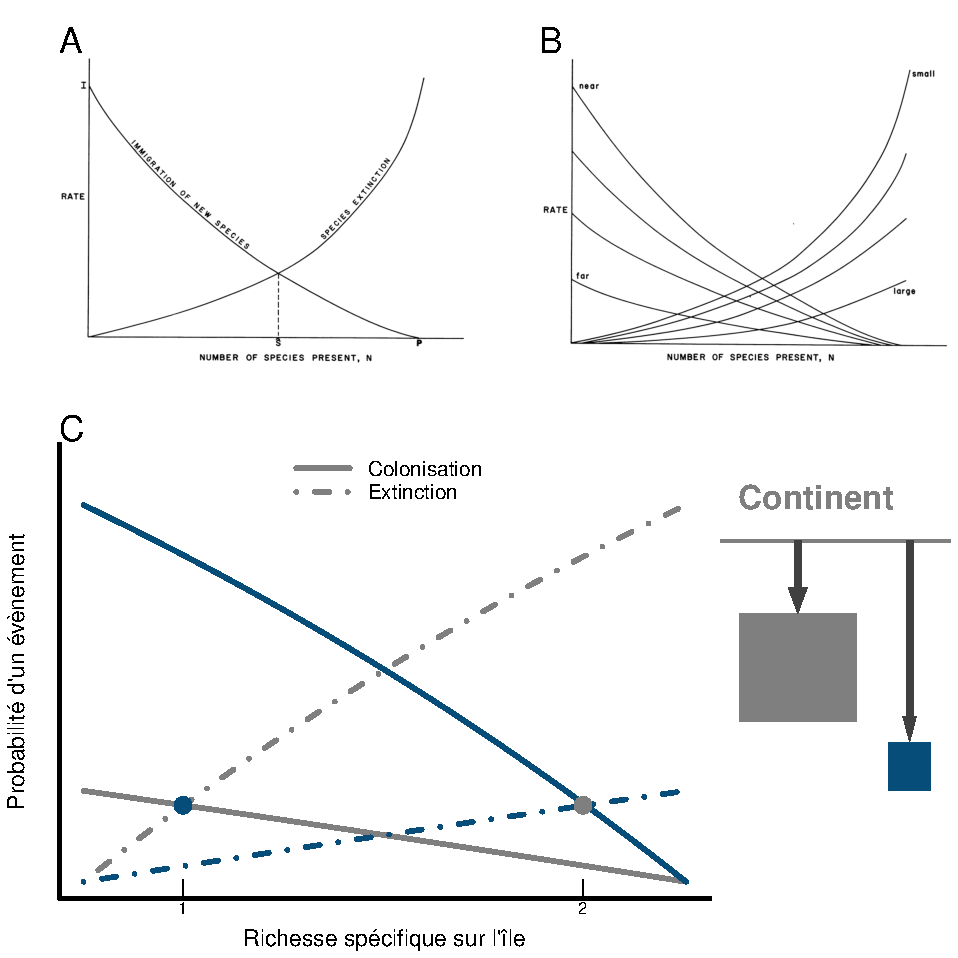
\includegraphics{fig/fig1.pdf}
\caption{\textbf{La Théorie de la biogéographie des Iles.} (A) illustre
l'évolution des taux de colonisation et d'extinction est présentée pour
deux îles aux caractéristiques différentes. Les tailles relatives des
îles et les distances qui les séparent du continent sont schématisées
sur la droite, les couleurs associent les îles à leur courbe respective.
Le pool d'espèce régional (\(P\)) est constitué de 100 espèces, les taux
de colonisation et d'extinction sont exprimés en terme de probabilité
d'un évènement (de colonisation ou d'extinction). Les points marquent
les intersecions entre les courbes d'extinction et de colonisation
c'est-à-dire lorsuqe ces processus s'équilibrent et pour lesquelles les
abscisses fournissent les richesses spécifiques de l'île à l'équiibre
\(S_{eq}\). (B) et (C) sont respectivement les figures 4 et 5 extraites
de l'article de 1963 de MacArthur et Wilson qui livre essentiellemnt le
même message que celui illustré en (A) (MacArthur and Wilson, 1963). La
forme convexe des courbes de 1963 sont justifiées par des facteurs
biologiques qui ne sont pas intégrés dans l'équation \label{eqMW} qui
confère une forme concave aux courbes comme vu en (A).\label{fig:figMW}}
\end{figure}

\subsubsection*{L'importance de la TIB dans des dévelopements théoriques
plus
récents}\label{limportance-de-la-tib-dans-des-duxe9velopements-thuxe9oriques-plus-ruxe9cents}
\addcontentsline{toc}{subsubsection}{L'importance de la TIB dans des
dévelopements théoriques plus récents}

\subsubsection*{La théorie des
métapopulations}\label{la-thuxe9orie-des-muxe9tapopulations}
\addcontentsline{toc}{subsubsection}{La théorie des métapopulations}

Bien que ne représentant que cinq pourcents des teres émergeés, ce sont
bien les observations de la faune des îles qui ont mené à une vision
paradigmatique de la biogéographie. L'importance des îles s'expliquent
par leur relative abondance, leur disparité, leur diversité, la relative
simplicité des assemblages biologiques qu'on y trouve et aussi, comme je
l'ai évoqué précedemment, par la clareté des flux de migrations
(Simberloff, 1974). Cette dernière propriété est souvent absente pour
des populations continentales\footnote{Les îles sont cependant souvent
  dans des archipels où la lecture de ces flux n'est pas si simple.}. La
théorie des métapopulations s'intéresse justement aux populations
reliées entre elles par des flux de migrations (Hanski, 2010). Le
premier modèle de métapopulations a été propopsé par Levins\footnote{Richard
  Levins qui avec Heatwole est un des co-découvreurs des idées de la
  TIB.} lors d'une réflexion sur le contrôle démographique des ravageurs
dans les cultures. Pour un ravageur donnée, les îlots de culture sont
autant de patchs où une population peut se maintenir et dispersé dans
les autres pacths alentour. Levins montre alors que les mesures de la
lutte biologique doivent être conduites à large échelle pour en
augmenter les probabilités de succès donc d'extinction régional du
ravageur~(Levins, 1969). Le modèle est simple et très proche de celui de
la TIB : l'évolution de la proportion \(p\) est aussi gouvernée par des
évènements de colonisation \(c\) et d'extinction \(e\) :

\begin{eqnarray}
\label{eqMW}
\frac{dp}{dt} = cp(1-p)-ep
\end{eqnarray}

La différence fondamentale avec la TIB est que la migration dépend de la
proportion de patchs occupés : plus elle est importante plus la
migration est importante. Parmis les démonstrations il y a les travaux
menés notamment par Ikkha Hanski sur les population du Mélitée du
plantain (\emph{Melitaea cinxia}) au sud-ouest de la Finland (Hanski,
1998). En plus de données un cadre de penser plus réaliste en terme de
configuration spatiale, les dynamiques populationnelles associées sont
bien expliquée et mènent à des risques d'extinction mieux cerner
(Hanski, 1998). C'est aussi un cadre aproprié pour insérer l'étude des
flux génétiques liés à l'arragment spatial des populations ainsi,
toujours sur ces mêmes populations de papillon Ilik Saccheri et
collègues montre qu'en ajoutant le degrés d'hétérozygotie, ils obteinnet
des proédictions précise auand à l'extinction locale des populations
(Saccheri et al., 1998). Les travaux théoriques autour du concept de
metapopulations proposent un certain nombre de paradigme qui permettent
d'évaluer le rôle que je joue les processus de colonisation et
d'extinction dans les variations spatio-temporelle de la démograohie
d'une espèce (Leibold et al., 2004). La prépondérance de ces mécanimes
qui font la force de la TIB et de la théorie des métatpopulation a été
poussé à son paroxysme dans la théorie neutre de la biogéographie.

\subsubsection*{La théorie neutre de la biogéographie et le débat
qu'elle
soulève}\label{la-thuxe9orie-neutre-de-la-bioguxe9ographie-et-le-duxe9bat-quelle-souluxe8ve}
\addcontentsline{toc}{subsubsection}{La théorie neutre de la
biogéographie et le débat qu'elle soulève}

La théorie neutre postule l'équivalence écologique entre les différents
individus d'espèces éventuellement différentes et décrit les dynamiques
populationnelles reposant sur les différences d'abondance relative à
l'échelle régionale et locale. Ainsi, en 1997, dans l'article fondateur
de la théorie neutre, Stephen Hubbell décrit un modèle dans lequel le
replacement d'un individu mort dans une communauté locale est le
résultat d'un tirage aléatoire : le nouvel individu peut soit être
recruté localement et la probabilité que l'individu soit d'une espèce
donnée dépend de l'abondance relative de cette dernière dans la
communauté locale soit le nouvel individu peut-être un immigrant dont
l'identité de l'espèce à laquelle il appartient est liée à l'abondance à
l'échelle régionale de celle-ci (Hubbell, 1997). En plus des exenples
données dans l'article de 1997, Hubbell montre de manière convaincante
que dans la foret tropical du Panama, à la suite d'un chablis, le
recrutement de l'arbre n'est pas prévisible par ces carctéritqiue et que
le recrutement est similaire à la composition alentour (Hubbell, 1999).
La dynamique engendrée est appelée la dérive écologique, elle dominée
par la stochasticité qui conduit preque certainement à l'extinction
presque certaine de toutes les espèces, ce qui est contrebalancée par
l'apparition d'espèces nouvelles (Hubbell, 2010, Ricklefs (2003)).

La théorie neutre partage beaucoup de charactéristiques avec la TIB : en
plus des principes fondamentaux d'extinction et de colonisation et du
d'équivalence écologique, elle impliqeu imbrication des échelles
régionales et locales. Comme le fait remarquer Hubbell en 2010 dans le
chapitre qu'il écrit dans \emph{The Theory of Island Biogeography
Revisited}, la théorie neutre place l'équivalence écologique au niveau
des individus et non plus au niveau des espèces (Hubbell, 2010). Une
conséquence directe revendiquée par Hubbell est que cette hypothèse
explique la forme convexe des courbes de colonisation et d'extinction
décrites par MacArthur et Wislon mais que n'explique pas leur modèle
(voir ({\textbf{???}}) et Hubbell (2010)). Le principe d'équivalence et
la palce importante que semble joué le hasard dans cette théorie a
soulevé de très vif débat avec des démonstrations à charge contre la
véracité de la théorie (voir par exemple McGill and Collins (2003) et
Ricklefs (2003)). A mon sens, l'équivalence écologique doit, comme dans
le cas de la TIB, être prise pour une abstraction de la sigularité des
espèces, une simplification de la diversité des systèmes biologiques,
pour isoler une portion restreinte des phénomènes qui la modifient pour
en évaluer finalement le pouvoir explicatif. Bien qu'un certain nombre
de cas d'études permettent de rejeter cette théorie (McGill and Collins,
2003, John et al. (2007)), les defenseurs de la théorie neutre affirment
qu'elle est tout aussi utile quand une étude en démontre la fausseté
(Rosindell et al., 2012). La théorie neutre peut en effet être présentée
comme une jauge qui mesure sur l'importance des processus de
différentiation de niches (Wennekes et al., 2012). Ainsi pour certaines
communauté la dérive écologique est plus importante que dans d'autre et
du point du vue de formalisme des solutions ont déjà été proposée pour
dresser un continuum de la théorie neutre vers la théorie de la niche
écologique (Gravel et al., 2006). Malgrés les possibilités offertent par
ces deux théories, elles occultent largement les interactions
écologiques qui sont factuelles; si les observations donnent crédit à
ces théories, une théorie intégrative de la biogéographie doit expliquer
pouquoi.

\section*{Le rôle des interactions dans la distribution des
espèces}\label{le-ruxf4le-des-interactions-dans-la-distribution-des-espuxe8ces}
\addcontentsline{toc}{section}{Le rôle des interactions dans la
distribution des espèces}

Ma thèse a pour objectif de trouver des leviers pour comprendre comment
les interactions peuvent affecter la répartition géographique des
espèces et de comprendre où chercher les traces qu'elles pourraient
éventuellement laisser dans les données d'occurrence des espèces. Comme
je l'ai mentionné plus haut cette idée est très ancienne, Wallace le
remarque dans son livre publié en 1881:

\begin{quote}
« Both competition and predation appear now to be much more important in
biogeography than people had formely guesses » (Wallace (1881) :28)
\end{quote}

Le problème de ces relations écologiques est leur spécificité, l'unicité
de chacune d'entre elle, dont découle nos difficultés pour les prévoir
bien que des travaux récents explorent des pistes prometeuse pour les
prédire notamment sur la base de relations allométriques entre proie et
prédateur (Gravel et al., 2013). Au point de vue théorique et à l'examen
des chapitres du dernier livre de MacArthur (MacArthur, 1972), on peut
que l'intégration des interactions est une étape clef pour aller vers
une biogéographie intégrative et c'est dans cette direction que j'ai
mené ma thèse en essayant d'apporter quelques pistes de reflexion.

\subsection*{Importance des interactions dans la
distribution}\label{importance-des-interactions-dans-la-distribution}
\addcontentsline{toc}{subsection}{Importance des interactions dans la
distribution}

Dans la théorie de la biogéographie des îles, les interactions sont en
fait omniprésentes car ells sont une des composantes principales du
processus d'extinction. Cependant dans la formulation du modèle, elles
ne sont jamis mentionnées explicitement, cachés dans le taux
d'extinction \(e\). Comme je le montre à la figure ({\textbf{???}}), la
différence dans l'allure des courbes déssinées par MacArthur et Wilson
et celles obtenues en suposant un taux d'immigration et de colonisation
sont différentes. D'après les auteurs, l'immigration devient plus
difficile lorsque les espèces s'accumulent sur l'île et les extinctions
sont de plus en plus fréquentes dues à l'intensification des
interactions. Pour parler en terme de réseau d'interaction,
l'accumulation d'espèces sur l'île sature le réseau local et rend
difficile l'intégration d'une nouvelle espèce et le rend de plus en plus
instable. Une interprétation en terme de communauté de la TIB est tout à
fait possible mais les liens entre les espèces ne sont pas formulés
mathématiquement en 1967.

Depuis les années 60, la litérature théorique n'a cessé de discuter le
rôle joué par les interactions intra- et inter-spécifiques dans la
distribution spatiale des espèces. Il est reconnu que l'interdépendance
des espèces conditionne, l'aspect favorable de l'environnement au sens
large (biotique et abiotique). En 2009, Robert Holt et Michael Barfield
discutent de l'impact de la prédation sur la répartition d'espèces en
compétition insistant alors sur le rôle majeur des interactions dans le
dessin des aires de répartition (Holt and Barfield, 2009). En 2012,
William Godsoe et Luke Harmon Godsoe introduisent les interactions dans
un modèle simple de distribution d'espèce et montre comment la
probabilité de présence d'une espèce peut être affectée par la
distribution d'une seconde et concluent que cela doit affecter
vraisemblablement la qualité de prédictions des SDMs (Godsoe and Harmon,
2012). Ils remettent alors en question ces derniers dotn triomphe à la
fin du siècle dernier avait relégué les interactions écologiques au
second plan en démontrant que la corrélation avec les variables
climatiques étaient peut-être suffisante, au moins en première
approximation pour expliquer les aires de répartitons (Pearson and
Dawson, 2003). Pourtant, dès 1998, le travail précurseur d'Andrew Davis
et collègues montrent que les interactions pourraient affectées nos
prédictions (Davis et al., 1998) remantant ainsi largement en cause
l'hypoythèse d'indépendance des espèces (Jeschke and Strayer, 2008).
L'expérience dont les résultats sont publié en 1998 est une annalyse
d'abondance de trois espèces de drospophile le long d'un gradient de
températive. Les comparaison d'abondance sont menées pour toues les
combinaisons possibles de ces trois mouches (assemblages à 1, 2 ou 3
espèces) mais aussi en présence ou en absence d'un parasitoïdes. La
démonstration est sans appel, la compétition et paraitsisme affectent
draistquement la survie le long du gradient de température, les
interactions affectent probablement les réponse au changements
climatqiue.

Plus récemment, on constate une grande motivation pour intégrer les
relations écologiques dans les modèles de distribution d'espèces
(Kissling et al., 2012, Guisan and Rahbek (2011)). Une méhodologie
récente appelée JSDM intègre par exemple les corrélations dans la
présence des espèces pour améliorer les prédictions (Pollock et al.,
2014). Néanmoins, ces efforts se heurtent à un manque de maturité des
modèles et théories qui cherchent à rassembler distribution et
interactions. Parmis les tarvaux récents, Franck Jabot et Jordi
Bascompte ont rassemblé metacommunautés et écologie des réseaux
souligner importance des relation écologique dans la répartition
géogrpahique des espèces (Jabot and Bascompte, 2012). De même, Dominique
Gravel et collègues introduisent en 2011 l'interdépendance
proie-prédateur dans le modèle de la TIB menant aux prémices d'une
théorie trophique de la biogéographie des îles (Gravel et al., 2011)
préfigurée par Holt (Holt, 2009).

C'est dans la lignée de ces développemnts théoriques récents que
s'inscrit mon premier chapitre de thèse. J'y ai montré comment
l'intégration du concept de réseau écologique dans la TIB était possible
tout en ajoutant la reconnaissance de performances plus ou moins
importantes des espèces dans un context abiotique donné (niche
écologique). Pour y arriver, j'ai montré l'interêt de ne pas considérer
des espèces une à une mais bien sous forme d'assemblage. Du point de vie
technique, mon travail montre aussi qu'un retour au processus
stochastique tels que ceux présentés en 1967 est une démarche puissante
pour ajouter des processus dans le modèle original.

\begin{figure}[htbp]
\centering
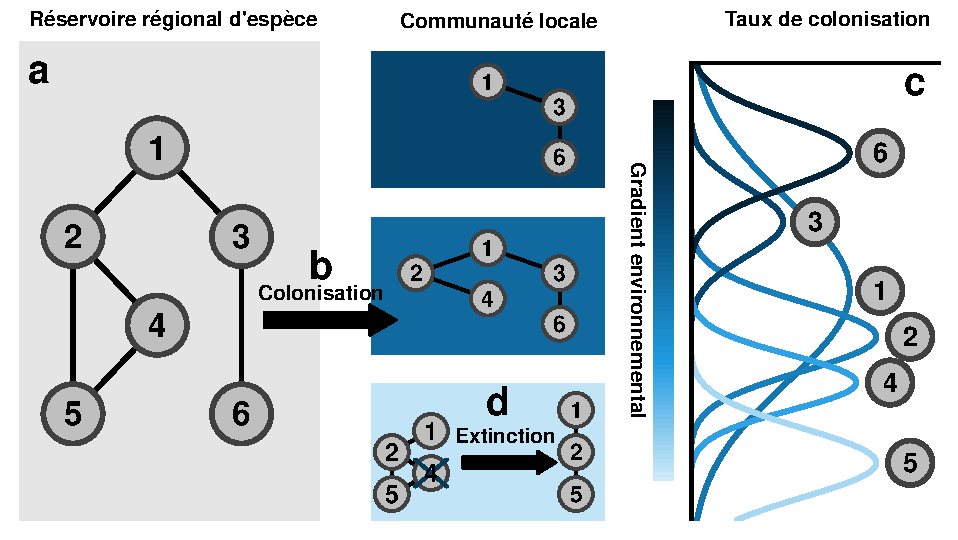
\includegraphics{fig/fig2.pdf}
\caption{\textbf{Intégration des interactions et des containtes
abiotiques dans la TIB.} Pour intégrer les interactions j'ai considéré
n'on pa un ensmeble d'espèce indépendant mais un des espèce au sein d'un
réseau décrit à l'échelle régional (a). Comme dans la TIB ces espèces
peuvent être colonisée l'île (b), mais dans le modèle que j'ai
développé, les taux de colonisation varient avec le long d'un gradient
environemntal (c). Enfin les interactions influencent les taux
d'extinction locaux (d).\label{fig:figGTIB}}
\end{figure}

\subsection*{Un problème d'échelle?}\label{un-probluxe8me-duxe9chelle}
\addcontentsline{toc}{subsection}{Un problème d'échelle?}

En repartant de l'exemple classique de la ségrégations spatiales des
tamias \emph{Eutamias dorsalis} et \emph{E. umbrinus} (Brown, 1971),
j'aiprécédemment mis en évidence qu'une information sur les interactions
contenus dans l'analyse des aires de répartitions. Il y a cependant deux
caractéristiques importantes qui peuvent faire obstacle à l'abondance de
ce type de lecture : la singularité de l'interaction et son caractère
locale. Je reviens un peu plus bas sur la première prpopriété et
m'arrête ici sur la seconde. Une idée forte relative aux interactions
est leur rôle majeur à l'échelle locale qui a des conséquences de moins
en moins perceptible au fur et à mesure que l'on cosidère des échelles
spatiales de plus en plus grande (voir l'unique figure de McGill
(2010)). Du point de vue théorique, c'est tout à fait ce qui est décrit
dans la TIB car c'est à l'échelle locale que les interactions
influencent l'extinction. Néanmoins, ces conséquences locales sont
présentent sur l'ensemble de la distribution de l'espèce, il est alors
pertient de se demander pourquoi nous ne sommes pas capables de detecter
les interactions en examinant les distributions d'espèces. En fait, nous
avons des preuves que cela est possible dans certains cas. En 2010,
Nicholas Gotelli et collègues divisent l'avifaune danoise en différentes
catégories fondées sur la similarité écologique et démontrent que les
espèces d'une même catégorie sont très souvent significativement
ségréguées (Gotelli et al., 2010). De même, en 2007, Risto Heikkinen et
collègues avaient ibtenu des performances accrues de leurs modèles
statisiques par l'utilisation de la répartition de six espèces de pics
pour expliquer la présence de quatre espèces de hiboux (Heikkinen et
al., 2007). Dans cette même étude, le signal est plus fort quand les
données sont sur de 10\emph{10km que 40}40km en faveur d'une dépendance
à l'échelle, récemment supportée par d'autres travaux (Belmaker et al.,
2015). Ce qui est remarquable dans les travaux de Gotelli et de
Heikkinen est que l'utilisation d'une connaissance biologique et
écologique a permis de révéler une trace des interaction dans la
distribution d'espèces.

La dépendance spatiale de la detection des intéractions est facile à
comprendre : en examinant des données de présence à des échelles
spatiales de plus en plus large, le nombre d'espèces s'accumule (c'est
le principe de la relation aire-espèce) menant à la dégradation de
l'information potentielle contenu dans différence plus locales. Cela
signifie que l'information nécessaire pour déceler des empreintes laissé
par les interactions sera fournit par des données à l'échelles
relativemnt dfine, cela ne permet pas de conclure sur le rayon d'action
de ces interactions. Pour dépasser la question spatiale, il fait aussi
envidagée l'impact de la nature des interactions sur la répartitin
géographique. Ainsi, en 2014, Miguel Araújo et Alejandro Rozenfeld ont
prouvé théoriquemnet que les les interactions positives (mutualisme) se
propageaient davantage que les intéractions négatives (Araújo and
Rozenfeld, 2014), la nature de la relation qui unie des espèces peut
donc influencer la perte d'information contenue dans les aire de
répartition. Suite à mes travaux sur l'intégrations des interactions, je
me suis penché sur un autre aspect qui peut influencer la perte
d'information dans dans les données de présence : l'abondance des
interactions. Au chapitre 2, je montre que les interactions directes et
indirectes affactent les données de distributions mais aussi que
l'abondance des interactions rend difficile de distinguer la
co-occurrence d'espèces en interactions d'une co-occurrence aléatoire.
Ce qui est encore plus intéressant, c'est que j'ai accumulé un un
certains nombre d'indices dans des données de présence et d'abscence
réelle qui semblent confirmer nos prédictions. Je discute de ces
résultats dans le troisième chapitre de ma thèse mon troisième chapitre.

En constant que l'abondance des interactions peut justifier l'hypothèse
d'indépendance des espèces, je soulève le même paradoxe que celui relevé
par MacArthur dans son oeuvre de 1972 (MacArthur, 1972) :

\begin{quote}
« A few decades ago it as fashionable for ecologist to study communities
in the arctic on the grounds that these would be very simple communities
and hence easy to understand. Many excellent ecologists still follow
this belied, but there are others who feel that it may be easier to
understand the extremely complex communities. This sounds paradoxical:
How can a more complex communities by easier to understand? A possible
answer might be that complex community has has strong interactions among
species so that the lives of the separate species are less independent
than in a simple community. Where there is greater interdependence,
patterns may be more conspicuous. »
\end{quote}

Encore une fois, je déplace le problème car si l'interdépendance est
importante pour des système smple, le porblème est de prédire aund ces
systèmes le sont. Autrement dit il serait peut-être pertinent de situer
les prédictions en biogéogrpahie au niveau du réseau écologique. Le
problème d'échelle n'est plus seulemnt spatial et temporel il est aussi
un problème d'échelle biologique : individus, population, communauté ou
réseaux?

\subsection*{Vers une biogéographie
énergétique}\label{vers-une-bioguxe9ographie-uxe9nerguxe9tique}
\addcontentsline{toc}{subsection}{Vers une biogéographie énergétique}

Le problème d'échelle biologique est aussi un problème de catégorisation
des espcèes. J'ai suggéré que les prédiction étaient plus facile pour
des espèces généralistes que pour des espèces spécialistes.
Malheureusement le spectre est très large et plutôt balancé avec un
continum entre des espèces hyperspécialistes de d'autres très
généralistes (Timothée Poisot et al., 2015). On peit néamoins espèrer
que la réduction des espèces à un certains nombres de traits (McGill et
al., 2006, T. Poisot et al. (2015)) et des réseaux à un certains nombre
de propriétés puissent permettrent des généralisations utiles dans notre
compréhension de leur distribution. Il m'apparaît aujourd'hui urgent que
le niveau bon niveau de détail dans nos descriptions des systèmes
écologiques soit trouvé afin de renforcer les fondements théoriques de
la dynamique des aires de répartitions.

Une piste prometteuse pour prolonger la recherche des propriétés est me
semble-t-il de s'appuyer sur la nature profonde des espèces : des
sytèmes énergétiques qui se perpétuent. La lecture de la théorie de la
dynamique du budget énergétique de Sebastian Kooijman (Kooijman, 2000)
m'a été très profitable pour cerner les possibilités offertes par une
telle approche. Si, comme il est montré par Kooijman, il est possible de
dériver de manière précise un grande nombre de propriétés énergétiques
des espèces sur leur masse et leur forme, alors les espoirs sont grands
de pouvoir trouver des règles d'assemblages fiables des commautés et
donc de comprendre d'un point de vue méchaniste les extinctions locales.
Ce sont les mêmes espoirs que ceux nourrit par la théorie métabolique de
l'écologie qui rassemble des relations entre la taille des espèces et
différentes de leurs propriétés (Brown et al., 2004) qui montrent en
somme qu'il est possible d'aller au dela de l'espèce (T. Poisot et al.,
2015). Mes reflexions sur l'intersection entre la TIB et une vision
énergétique de l'écologue sont présentées au chapitre 4 de ma thèse,
dans un chapitre qui se veut aussi comme une ouverture vers les projets
de recherche que j'aimerais mener dans un futur proche.

\hypertarget{refs}{}
\hypertarget{ref-Allesina2012a}{}
Allesina, S., Tang, S., 2012. Stability criteria for complex ecosystems.
Nature 483, 205--208.
doi:\href{https://doi.org/10.1038/nature10832}{10.1038/nature10832}

\hypertarget{ref-TheArabidopsisGenomeInitiative2000}{}
Arabidopsis Genome Initiative, 2000. Analysis of the genome sequence of
the flowering plant Arabidopsis thaliana. Nature 408, 796--815.
doi:\href{https://doi.org/10.1038/35048692}{10.1038/35048692}

\hypertarget{ref-Araujo2014}{}
Araújo, M.B., Rozenfeld, A., 2014. The geographic scaling of biotic
interactions. Ecography 37, 406--415.
doi:\href{https://doi.org/10.1111/j.1600-0587.2013.00643.x}{10.1111/j.1600-0587.2013.00643.x}

\hypertarget{ref-Balanya2006}{}
Balanyá, J., Oller, J.M., Huey, R.B., Gilchrist, G.W., Serra, L., 2006.
Global genetic change tracks global climate warming in Drosophila
subobscura. Science (New York, N.Y.) 313, 1773--5.
doi:\href{https://doi.org/10.1126/science.1131002}{10.1126/science.1131002}

\hypertarget{ref-Beck2012}{}
Beck, J., Ballesteros-Mejia, L., Buchmann, C.M., Dengler, J., Fritz,
S.A., Gruber, B., Hof, C., Jansen, F., Knapp, S., Kreft, H., Schneider,
A.-K., Winter, M., Dormann, C.F., 2012. What's on the horizon for
macroecology? Ecography 35, 001--011.
doi:\href{https://doi.org/10.1111/j.1600-0587.2012.07364.x}{10.1111/j.1600-0587.2012.07364.x}

\hypertarget{ref-Beck2014a}{}
Beck, J., Böller, M., Erhardt, A., Schwanghart, W., 2014. Spatial bias
in the GBIF database and its effect on modeling species' geographic
distributions. Ecological Informatics 19, 10--15.
doi:\href{https://doi.org/10.1016/j.ecoinf.2013.11.002}{10.1016/j.ecoinf.2013.11.002}

\hypertarget{ref-Bellard2012}{}
Bellard, C., Bertelsmeier, C., Leadley, P., Thuiller, W., Courchamp, F.,
2012. Impacts of climate change on the future of biodiversity. Ecology
letters 15, 365--377.
doi:\href{https://doi.org/10.1111/j.1461-0248.2011.01736.x}{10.1111/j.1461-0248.2011.01736.x}

\hypertarget{ref-Belmaker2015}{}
Belmaker, J., Zarnetske, P., Tuanmu, M.-N., Zonneveld, S., Record, S.,
Strecker, A., Beaudrot, L., 2015. Empirical evidence for the scale
dependence of biotic interactions. Global Ecology and Biogeography 24,
750--761.
doi:\href{https://doi.org/10.1111/geb.12311}{10.1111/geb.12311}

\hypertarget{ref-Brown1971}{}
Brown, J.H., 1971. Mechanisms of Competitive Exclusion Between Two
Species of Chipmunks. Ecology 52, 305--311.
doi:\href{https://doi.org/10.2307/1934589}{10.2307/1934589}

\hypertarget{ref-Brown2004}{}
Brown, J.H., Gillooly, J.F., Allen, A.P., Savage, V.M., West, G.B.,
2004. Toward a metabolic theory of ecology. Ecology 85, 1771--1789.
doi:\href{https://doi.org/10.1890/03-9000}{10.1890/03-9000}

\hypertarget{ref-Brown1989}{}
Brown, J.H., Lomolino, M.V., 1989. Independent Discovery of the
Equilibrium Theory of Island Biogeography. Ecology 70, 1954--1957.
doi:\href{https://doi.org/10.2307/1938125}{10.2307/1938125}

\hypertarget{ref-Chase2003}{}
Chase, J.M., Leibold, M.A., 2003. Ecological niches : linking classical
and contemporary approaches.
doi:\href{https://doi.org/10.1007/s13398-014-0173-7.2}{10.1007/s13398-014-0173-7.2}

\hypertarget{ref-Connor1979}{}
Connor, E.F., Simberloff, D., 1979. The Assembly of Species Communities:
Chance or Competition? Ecology 60, 1132.
doi:\href{https://doi.org/10.2307/1936961}{10.2307/1936961}

\hypertarget{ref-Cook2002}{}
Cook, W.M., Lane, K.T., Foster, B.L., Holt, R.D., 2002. Island theory,
matrix effects and species richness patterns in habitat fragments.
Ecology Letters 5, 619--623.
doi:\href{https://doi.org/10.1046/j.1461-0248.2002.00366.x}{10.1046/j.1461-0248.2002.00366.x}

\hypertarget{ref-Davis1998}{}
Davis, A.J., Jenkinson, L.S., Lawton, J.H., Shorrocks, B., Wood, S.,
1998. Making mistakes when predicting shifts in species range in
response to global warming. Nature 391, 783--786.
doi:\href{https://doi.org/10.1038/35842}{10.1038/35842}

\hypertarget{ref-Desmet2004}{}
Desmet, P., Cowling, R., 2004. Using the species-area relationship to
set baseline targets for conservation. Ecology And Society 9, 1--39.

\hypertarget{ref-Diamond1975}{}
Diamond, J.M., 1975. Assembly of species communities, in: Cody, M.L.,
Diamond, J.M. (Eds.), Ecology and Evolution of Communities. Harvard
University Press, Cambridge, Massachusetts, USA., pp. 342--444.

\hypertarget{ref-Dobzhansky1973}{}
Dobzhansky, T., 1973. Nothing in Biology Makes Sense except in the Light
of Evolution. The American Biology Teacher 35, 125--129.
doi:\href{https://doi.org/10.2307/4444260}{10.2307/4444260}

\hypertarget{ref-Elith2006}{}
Elith, J., H. Graham, C., P. Anderson, R., Dudík, M., Ferrier, S.,
Guisan, A., J. Hijmans, R., Huettmann, F., R. Leathwick, J., Lehmann,
A., Li, J., G. Lohmann, L., A. Loiselle, B., Manion, G., Moritz, C.,
Nakamura, M., Nakazawa, Y., McC. M. Overton, J., Townsend Peterson, A.,
J. Phillips, S., Richardson, K., Scachetti-Pereira, R., E. Schapire, R.,
Soberón, J., Williams, S., S. Wisz, M., E. Zimmermann, N., 2006. Novel
methods improve prediction of species' distributions from occurrence
data. Ecography 29, 129--151.
doi:\href{https://doi.org/10.1111/j.2006.0906-7590.04596.x}{10.1111/j.2006.0906-7590.04596.x}

\hypertarget{ref-Elith2009a}{}
Elith, J., Leathwick, J.R., 2009. Species Distribution Models:
Ecological Explanation and Prediction Across Space and Time. Annual
Review of Ecology, Evolution, and Systematics 40, 677--697.
doi:\href{https://doi.org/10.1146/annurev.ecolsys.110308.120159}{10.1146/annurev.ecolsys.110308.120159}

\hypertarget{ref-Engelbrecht2007}{}
Engelbrecht, B.M.J., Comita, L.S., Condit, R., Kursar, T. a, Tyree,
M.T., Turner, B.L., Hubbell, S.P., 2007. Drought sensitivity shapes
species distribution patterns in tropical forests. Nature 447, 80--82.
doi:\href{https://doi.org/10.1038/nature05747}{10.1038/nature05747}

\hypertarget{ref-Finstermeier2013}{}
Finstermeier, K., Zinner, D., Brameier, M., Meyer, M., Kreuz, E.,
Hofreiter, M., Roos, C., 2013. A Mitogenomic Phylogeny of Living
Primates. PLoS ONE 8, 1--10.
doi:\href{https://doi.org/10.1371/journal.pone.0069504}{10.1371/journal.pone.0069504}

\hypertarget{ref-Godsoe2012}{}
Godsoe, W., Harmon, L.J., 2012. How do species interactions affect
species distribution models? Ecography 35, 811--820.
doi:\href{https://doi.org/10.1111/j.1600-0587.2011.07103.x}{10.1111/j.1600-0587.2011.07103.x}

\hypertarget{ref-Gotelli2010}{}
Gotelli, N.J., Graves, G.R., Rahbek, C., 2010. Macroecological signals
of species interactions in the Danish avifauna. Proceedings of the
National Academy of Sciences 107, 5030--5035.
doi:\href{https://doi.org/10.1073/pnas.0914089107}{10.1073/pnas.0914089107}

\hypertarget{ref-grant2008}{}
Grant, P.R., Grant, B.R., 2008. How and Why Species Multiply: The
Radiation of Darwin's Finches, Princeton series in evolutionary biology.
Princeton University Press.

\hypertarget{ref-Gravel2006a}{}
Gravel, D., Canham, C.D., Beaudet, M., Messier, C., 2006. Reconciling
niche and neutrality: the continuum hypothesis. Ecology letters 9,
399--409.
doi:\href{https://doi.org/10.1111/j.1461-0248.2006.00884.x}{10.1111/j.1461-0248.2006.00884.x}

\hypertarget{ref-Gravel2011}{}
Gravel, D., Massol, F., Canard, E., Mouillot, D., Mouquet, N., 2011.
Trophic theory of island biogeography. Ecology Letters 14, 1010--1016.
doi:\href{https://doi.org/10.1111/j.1461-0248.2011.01667.x}{10.1111/j.1461-0248.2011.01667.x}

\hypertarget{ref-Gravel2013a}{}
Gravel, D., Poisot, T., Albouy, C., Velez, L., Mouillot, D., 2013.
Inferring food web structure from predator-prey body size relationships.
Methods in Ecology and Evolution 4, 1083--1090.
doi:\href{https://doi.org/10.1111/2041-210X.12103}{10.1111/2041-210X.12103}

\hypertarget{ref-Grinnell1917a}{}
Grinnell, J., 1917. The Niche-Relationships of the California Thrasher.
The Auk 34, 427--433.
doi:\href{https://doi.org/10.2307/4072271}{10.2307/4072271}

\hypertarget{ref-Guisan2011}{}
Guisan, A., Rahbek, C., 2011. SESAM - a new framework integrating
macroecological and species distribution models for predicting
spatio-temporal patterns of species assemblages. Journal of Biogeography
38, 1433--1444.
doi:\href{https://doi.org/10.1111/j.1365-2699.2011.02550.x}{10.1111/j.1365-2699.2011.02550.x}

\hypertarget{ref-Hannah2013}{}
Hannah, L., Roehrdanz, P.R., Ikegami, M., Shepard, A.V., Shaw, M.R.,
Tabor, G., Zhi, L., Marquet, P.a., Hijmans, R.J., 2013. Climate change,
wine, and conservation. Proceedings of the National Academy of Sciences
110, 6907--6912.
doi:\href{https://doi.org/10.1073/pnas.1210127110}{10.1073/pnas.1210127110}

\hypertarget{ref-Hanski2010}{}
Hanski, I., 2010. The Theories of Island Biogeography and Metapopulation
Dynamics, in: The Theory of Island Biogeography Revisited. Princeton
University Press, Princeton, NJ, p. 476.

\hypertarget{ref-Hanski1998}{}
Hanski, I., 1998. Metapopulation dynamics. Nature reviews 396, 41--49.
doi:\href{https://doi.org/10.1016/0169-5347(89)90061-X}{10.1016/0169-5347(89)90061-X}

\hypertarget{ref-He2011}{}
He, F., Hubbell, S.P., 2011. Species-area relationships always
overestimate extinction rates from habitat loss. Nature 473, 368--71.
doi:\href{https://doi.org/10.1038/nature09985}{10.1038/nature09985}

\hypertarget{ref-Heikkinen2007}{}
Heikkinen, R.K., Luoto, M., Virkkala, R., Pearson, R.G., Körber, J.-H.,
2007. Biotic interactions improve prediction of boreal bird
distributions at macro-scales. Global Ecology and Biogeography 16,
754--763.
doi:\href{https://doi.org/10.1111/j.1466-8238.2007.00345.x}{10.1111/j.1466-8238.2007.00345.x}

\hypertarget{ref-Hijmans2005}{}
Hijmans, R.J., Cameron, S.E., Parra, J.L., Jones, P.G., Jarvis, A.,
2005. Very high resolution interpolated climate surfaces for global land
areas. International Journal of Climatology 25, 1965--1978.
doi:\href{https://doi.org/10.1002/joc.1276}{10.1002/joc.1276}

\hypertarget{ref-Holt2009a}{}
Holt, R.D., 2009. Bringing the Hutchinsonian niche into the 21st
century: ecological and evolutionary perspectives. Proceedings of the
National Academy of Sciences of the United States of America 106 Suppl,
19659--65.
doi:\href{https://doi.org/10.1073/pnas.0905137106}{10.1073/pnas.0905137106}

\hypertarget{ref-Holt2009}{}
Holt, R.D., Barfield, M., 2009. Trophic interactions and range limits:
the diverse roles of predation. Proceedings. Biological sciences / The
Royal Society 276, 1435--1442.
doi:\href{https://doi.org/10.1098/rspb.2008.1536}{10.1098/rspb.2008.1536}

\hypertarget{ref-Hortal2011}{}
Hortal, J., Diniz-Filho, J.A.F., Bini, L.M., Rodríguez, M.Á., Baselga,
A., Nogués-Bravo, D., Rangel, T.F., Hawkins, B.A., Lobo, J.M., 2011. Ice
age climate, evolutionary constraints and diversity patterns of European
dung beetles. Ecology Letters 14, 741--748.
doi:\href{https://doi.org/10.1111/j.1461-0248.2011.01634.x}{10.1111/j.1461-0248.2011.01634.x}

\hypertarget{ref-Hubbell2010}{}
Hubbell, S.P., 2010. Neutral Theory and the Theory of Island
Biogeography, in: Losos, J.B., Ricklefs, R.E. (Eds.), The Theory of
Island Biogeography Revisited. Princeton University Press, Princeton,
NJ, p. 479.

\hypertarget{ref-Hubbell1999}{}
Hubbell, S.P., 1999. Light-Gap Disturbances, Recruitment Limitation, and
Tree Diversity in a Neotropical Forest. Science 283, 554--557.
doi:\href{https://doi.org/10.1126/science.283.5401.554}{10.1126/science.283.5401.554}

\hypertarget{ref-Hubbell1997}{}
Hubbell, S.P., 1997. A unified theory of biogeography and relative
species abundance and its application to tropical rain forests and coral
reefs. Coral Reefs 16, S9--S21.
doi:\href{https://doi.org/10.1007/s003380050237}{10.1007/s003380050237}

\hypertarget{ref-Jabot2012}{}
Jabot, F., Bascompte, J., 2012. Bitrophic interactions shape
biodiversity in space. Proceedings of the National Academy of Sciences
of the United States of America 109, 4521--4526.
doi:\href{https://doi.org/10.1073/pnas.1107004109}{10.1073/pnas.1107004109}

\hypertarget{ref-Jeschke2008}{}
Jeschke, J.M., Strayer, D.L., 2008. Usefulness of bioclimatic models for
studying climate change and invasive species. Annals of the New York
Academy of Sciences 1134, 1--24.
doi:\href{https://doi.org/10.1196/annals.1439.002}{10.1196/annals.1439.002}

\hypertarget{ref-John2007}{}
John, R., Dalling, J.W., Harms, K.E., Yavitt, J.B., Stallard, R.F.,
Mirabello, M., Hubbell, S.P., Valencia, R., Navarrete, H., Vallejo, M.,
Foster, R.B., 2007. Soil nutrients influence spatial distributions of
tropical tree species. Proceedings of the National Academy of Sciences
104, 864--869.
doi:\href{https://doi.org/10.1073/pnas.0604666104}{10.1073/pnas.0604666104}

\hypertarget{ref-Kearney2004}{}
Kearney, M., Porter, W.P., 2004. MAPPING THE FUNDAMENTAL NICHE:
PHYSIOLOGY, CLIMATE, AND THE DISTRIBUTION OF A NOCTURNAL LIZARD. Ecology
85, 3119--3131.
doi:\href{https://doi.org/10.1890/03-0820}{10.1890/03-0820}

\hypertarget{ref-Kefi2015}{}
Kéfi, S., Berlow, E.L., Wieters, E.A., Joppa, L.N., Wood, S.A., Brose,
U., Navarrete, S.A., 2015. Network structure beyond food webs: mapping
non-trophic and trophic interactions on Chilean rocky shores. Ecology
96, 291--303.
doi:\href{https://doi.org/10.1890/13-1424.1}{10.1890/13-1424.1}

\hypertarget{ref-Kefi2012}{}
Kéfi, S., Berlow, E.L., Wieters, E.A., Navarrete, S.A., Petchey, O.L.,
Wood, S.A., Boit, A., Joppa, L.N., Lafferty, K.D., Williams, R.J.,
Martinez, N.D., Menge, B.A., Blanchette, C.A., Iles, A.C., Brose, U.,
2012. More than a meal\ldots{} integrating non-feeding interactions into
food webs. Ecology Letters 15, 291--300.
doi:\href{https://doi.org/10.1111/j.1461-0248.2011.01732.x}{10.1111/j.1461-0248.2011.01732.x}

\hypertarget{ref-Kissling2011}{}
Kissling, W.D., Dormann, C.F., Groeneveld, J., Hickler, T., Kühn, I.,
McInerny, G.J., Montoya, J.M., Römermann, C., Schiffers, K., Schurr,
F.M., Singer, A., Svenning, J.-C., Zimmermann, N.E., O'Hara, R.B., 2012.
Towards novel approaches to modelling biotic interactions in
multispecies assemblages at large spatial extents. Journal of
Biogeography 39, 2163--2178.
doi:\href{https://doi.org/10.1111/j.1365-2699.2011.02663.x}{10.1111/j.1365-2699.2011.02663.x}

\hypertarget{ref-Koh2004}{}
Koh, L.P., 2004. Species Coextinctions and the Biodiversity Crisis.
Science 305, 1632--1634.
doi:\href{https://doi.org/10.1126/science.1101101}{10.1126/science.1101101}

\hypertarget{ref-Kooijman2000a}{}
Kooijman, S.A.L.M., 2000. Dynamic Energy and Mass Budgets in Biological
Systems. Cambridge University Press, Cambridge.
doi:\href{https://doi.org/10.1017/CBO9780511565403}{10.1017/CBO9780511565403}

\hypertarget{ref-Lavergne2010}{}
Lavergne, S., Mouquet, N., Thuiller, W., Ronce, O., 2010. Biodiversity
and Climate Change: Integrating Evolutionary and Ecological Responses of
Species and Communities. Annual Review of Ecology, Evolution, and
Systematics 41, 321--350.
doi:\href{https://doi.org/10.1146/annurev-ecolsys-102209-144628}{10.1146/annurev-ecolsys-102209-144628}

\hypertarget{ref-Leibold2004}{}
Leibold, M.a., Holyoak, M., Mouquet, N., Amarasekare, P., Chase, J.M.,
Hoopes, M.F., Holt, R.D., Shurin, J.B., Law, R., Tilman, D., Loreau, M.,
Gonzalez, a., 2004. The metacommunity concept: a framework for
multi-scale community ecology. Ecology Letters 7, 601--613.
doi:\href{https://doi.org/10.1111/j.1461-0248.2004.00608.x}{10.1111/j.1461-0248.2004.00608.x}

\hypertarget{ref-Levins1969}{}
Levins, R., 1969. Some Demographic and Genetic Consequences of
Environmental Heterogeneity for Biological Control. Bulletin of the
Entomological Society of America 15, 237--240.
doi:\href{https://doi.org/10.1093/besa/15.3.237}{10.1093/besa/15.3.237}

\hypertarget{ref-Levins1963}{}
Levins, R., Heatwole, H., 1963. On the distribution of organisms on
islands. Caribbean Journal of Science 3, 173--177.

\hypertarget{ref-Lomolino2000a}{}
Lomolino, M., 2000. Ecology's most general, yet protean pattern : the
species area relationship. Journal of Biogeography 27, 17--26.

\hypertarget{ref-Lomolino2000}{}
Lomolino, M.V., 2000. A call for a new paradigm of island biogeography.
Global Ecology and Biogeography 9, 1--6.
doi:\href{https://doi.org/10.1046/j.1365-2699.2000.00185.x}{10.1046/j.1365-2699.2000.00185.x}

\hypertarget{ref-Lomolino2009}{}
Lomolino, M.V., Brown, J.H., 2009. The reticulating phylogeny of island
biogeography theory. Q. Rev. Biol. 84, 357--390.
doi:\href{https://doi.org/10.1017/CBO9781107415324.004}{10.1017/CBO9781107415324.004}

\hypertarget{ref-Losos2010}{}
Losos, J.B., Ricklefs, R.E., 2010. The Theory of Island Biogeography
Revisited. Princeton University Press, Princeton, NJ.

\hypertarget{ref-macarthur1972geographical}{}
MacArthur, R.H., 1972. Geographical Ecology: Patterns in the
Distribution of Species, Biology / {[}princeton university press{]}.
Princeton University Press.

\hypertarget{ref-MacArthur1967}{}
MacArthur, R.H., Wilson, E.O., 1967. Theory of Island Biogeography,
Princeton landmarks in biology. Princeton University Press, Princeton,
NJ.

\hypertarget{ref-MacArthur1963}{}
MacArthur, R.H., Wilson, E.O., 1963. An equilibrium theory of insular
zoogeography. Evolution 17, 373--387.

\hypertarget{ref-MacArthur1967a}{}
MacArthur, R.H., Wilson, E.O., MacArthur, W., 1967. The theory of island
biogeography.
doi:\href{https://doi.org/10.2307/1796430}{10.2307/1796430}

\hypertarget{ref-May2004}{}
May, R.M., 2004. Uses and abuses of mathematics in biology. Science (New
York, N.Y.) 303, 790--3.
doi:\href{https://doi.org/10.1126/science.1094442}{10.1126/science.1094442}

\hypertarget{ref-May1973}{}
May, R.M., 1973. Stability and complexity in model ecosystems.
Monographs in population biology 6, 1--235.
doi:\href{https://doi.org/10.1109/TSMC.1978.4309856}{10.1109/TSMC.1978.4309856}

\hypertarget{ref-mccann2011food}{}
McCann, K.S., 2011. Food Webs, Monographs in population biology.
Princeton University Press.

\hypertarget{ref-McCann2000}{}
McCann, K.S., 2000. The diversity-stability debate. Nature 405, 228--33.
doi:\href{https://doi.org/10.1038/35012234}{10.1038/35012234}

\hypertarget{ref-McGill2003}{}
McGill, B., Collins, C., 2003. A unified theory for macroecology based
on spatial patterns of abundance. Evolutionary Ecology Research 5,
469--492.
doi:\href{https://doi.org/10.1038/nature01569.1.}{10.1038/nature01569.1.}

\hypertarget{ref-McGill2010}{}
McGill, B.J., 2010. Matters of Scale. Science 328, 575--576.
doi:\href{https://doi.org/10.1126/science.1188528}{10.1126/science.1188528}

\hypertarget{ref-McGill2006}{}
McGill, B.J., Enquist, B.J., Weiher, E., Westoby, M., 2006. Rebuilding
community ecology from functional traits. Trends in ecology \& evolution
21, 178--185.
doi:\href{https://doi.org/10.1016/j.tree.2006.02.002}{10.1016/j.tree.2006.02.002}

\hypertarget{ref-monod1970hasard}{}
Monod, J., 1970. Le hasard et la n\{é\}c\{é\}ssit\{é\}: Editions Du
Seuil.

\hypertarget{ref-Neigel2003}{}
Neigel, J., 2003. Species-area relatioships and marine conservation.
Ecological Applications 13, 138--145.
doi:\href{https://doi.org/10.1890/1051-0761(2003)013\%5B0138:SARAMC\%5D2.0.CO;2}{10.1890/1051-0761(2003)013{[}0138:SARAMC{]}2.0.CO;2}

\hypertarget{ref-Pearson2003}{}
Pearson, R.G., Dawson, T.P., 2003. Predicting the impacts of climate
change on the distribution of species: are bioclimate envelope models
useful? Global Ecology and Biogeography 12, 361--371.
doi:\href{https://doi.org/10.1046/j.1466-822X.2003.00042.x}{10.1046/j.1466-822X.2003.00042.x}

\hypertarget{ref-Pelletier2007}{}
Pelletier, F., Clutton-Brock, T., Pemberton, J., Tuljapurkar, S.,
Coulson, T., 2007. The evolutionary demography of ecological change:
Linking trait variation and population growth. Science 315, 1571--1574.
doi:\href{https://doi.org/10.1126/science.1139024}{10.1126/science.1139024}

\hypertarget{ref-Pelletier2009}{}
Pelletier, F., Garant, D., Hendry, a P., 2009. Eco-evolutionary
dynamics. Philosophical transactions of the Royal Society of London.
Series B, Biological sciences 364, 1483--9.
doi:\href{https://doi.org/10.1098/rstb.2009.0027}{10.1098/rstb.2009.0027}

\hypertarget{ref-Pelletier2009a}{}
Pelletier, F., Garant, D., Hendry, A., 2009. Eco-evolutionary dynamics.
Philosophical Transactions of the Royal Society B: Biological Sciences
364, 1483--1489.
doi:\href{https://doi.org/10.1098/rstb.2009.0027}{10.1098/rstb.2009.0027}

\hypertarget{ref-Poisot2015c}{}
Poisot, T., Kéfi, S., Morand, S., Stanko, M., Marquet, P.A., Hochberg,
M.E., 2015. A continuum of specialists and generalists in empirical
communities. PLoS ONE 10, 1--12.
doi:\href{https://doi.org/10.1371/journal.pone.0114674}{10.1371/journal.pone.0114674}

\hypertarget{ref-Poisot2015}{}
Poisot, T., Stouffer, D.B., Gravel, D., 2015. Beyond species: why
ecological interactions vary through space and time. Oikos 124,
243--251. doi:\href{https://doi.org/10.1101/001677}{10.1101/001677}

\hypertarget{ref-Pollock2014}{}
Pollock, L.J., Tingley, R., Morris, W.K., Golding, N., O'Hara, R.B.,
Parris, K.M., Vesk, P.A., McCarthy, M.A., 2014. Understanding
co-occurrence by modelling species simultaneously with a Joint Species
Distribution Model (JSDM). Methods in Ecology and Evolution 5, 397--406.
doi:\href{https://doi.org/10.1111/2041-210X.12180}{10.1111/2041-210X.12180}

\hypertarget{ref-Post2009}{}
Post, D.M., Palkovacs, E.P., 2009. Eco-evolutionary feedbacks in
community and ecosystem ecology: interactions between the ecological
theatre and the evolutionary play. Philosophical transactions of the
Royal Society of London. Series B, Biological sciences 364, 1629--40.
doi:\href{https://doi.org/10.1098/rstb.2009.0012}{10.1098/rstb.2009.0012}

\hypertarget{ref-Rcoreteam2015}{}
R Core Team, 2015. R: A Language and Environment for Statistical
Computing.

\hypertarget{ref-Razafindratsima2013}{}
Razafindratsima, O.H., Mehtani, S., Dunham, A.E., 2013. Extinctions,
traits and phylogenetic community structure: Insights from primate
assemblages in Madagascar. Ecography 36, 047--056.
doi:\href{https://doi.org/10.1111/j.1600-0587.2011.07409.x}{10.1111/j.1600-0587.2011.07409.x}

\hypertarget{ref-Ricklefs2003}{}
Ricklefs, R.E., 2003. A comment on Hubbell 's zero-sum ecological drift
model. Oikos 1001, 185--192.

\hypertarget{ref-Ricklefs1987}{}
Ricklefs, R.E., 1987. Community diversity: relative roles of local and
regional processes. Science 235, 167--171.
doi:\href{https://doi.org/10.1126/science.235.4785.167}{10.1126/science.235.4785.167}

\hypertarget{ref-Robinet2016}{}
Robinet, C., Suppo, C., Darrouzet, E., 2016. Rapid spread of the
invasive yellow-legged hornet in France: the role of human-mediated
dispersal and the effects of control measures. Journal of Applied
Ecology.
doi:\href{https://doi.org/10.1111/1365-2664.12724}{10.1111/1365-2664.12724}

\hypertarget{ref-Rosindell2012}{}
Rosindell, J., Hubbell, S.P., He, F., Harmon, L.J., Etienne, R.S., 2012.
The case for ecological neutral theory. Trends in Ecology and Evolution
27, 203--208.
doi:\href{https://doi.org/10.1016/j.tree.2012.01.004}{10.1016/j.tree.2012.01.004}

\hypertarget{ref-Saccheri1998}{}
Saccheri, I., Kuussaari, M., Kankare, M., Vikman, P., Fortelius, W.,
Hanski, I., 1998. Inbreeding and extinction in a butterfly
metapopulation. Nature 392, 491--494.
doi:\href{https://doi.org/Doi\%2010.1038/33136}{Doi 10.1038/33136}

\hypertarget{ref-Schoener2011a}{}
Schoener, T.W., 2011a. The Newest Synthesis : Understanding Ecological
Dynamics. Science 331, 426--429.
doi:\href{https://doi.org/10.1126/science.1193954}{10.1126/science.1193954}

\hypertarget{ref-Schoener2011}{}
Schoener, T.W., 2011b. The newest synthesis: understanding the interplay
of evolutionary and ecological dynamics. Science (New York, N.Y.) 331,
426--9.
doi:\href{https://doi.org/10.1126/science.1193954}{10.1126/science.1193954}

\hypertarget{ref-Sexton2009}{}
Sexton, J.P., McIntyre, P.J., Angert, A.L., Rice, K.J., 2009. Evolution
and Ecology of Species Range Limits. Annual Review of Ecology,
Evolution, and Systematics 40, 415--436.
doi:\href{https://doi.org/10.1146/annurev.ecolsys.110308.120317}{10.1146/annurev.ecolsys.110308.120317}

\hypertarget{ref-Simberloff1974a}{}
Simberloff, D.S., 1974. Equilibrium Theory of Island Biogeography and
Ecology. Annual Review of Ecology and Systematics 5, 161--182.
doi:\href{https://doi.org/10.1146/annurev.es.05.110174.001113}{10.1146/annurev.es.05.110174.001113}

\hypertarget{ref-Simberloff1969}{}
Simberloff, D.S., Wilson, E.O., 1969. Experimental Zoogeography of
Islands: The Colonization of Empty Islands. Ecology 50, 278--296.
doi:\href{https://doi.org/10.2307/1934856}{10.2307/1934856}

\hypertarget{ref-Simberloff1969a}{}
Simberloff, D.S., Wilson, E.O., 1969. Experimental zoogeography of
islands: a model for insular colonization. Ecology 50, 296--314.
doi:\href{https://doi.org/10.2307/1934856}{10.2307/1934856}

\hypertarget{ref-Springer2015}{}
Springer, A., Swann, D., Crimmins, M., 2015. Climate change impacts on
high elevation saguaro range expansion. Journal of Arid Environments
116, 57--62.
doi:\href{https://doi.org/10.1016/j.jaridenv.2015.02.004}{10.1016/j.jaridenv.2015.02.004}

\hypertarget{ref-Tao2010}{}
Tao, T., Vu, V., Krishnapur, M., 2010. Random matrices: Universality of
ESDs and the circular law. The Annals of Probability 38, 2023--2065.
doi:\href{https://doi.org/10.1214/10-AOP534}{10.1214/10-AOP534}

\hypertarget{ref-Thuiller2013}{}
Thuiller, W., Münkemüller, T., Lavergne, S., Mouillot, D., Mouquet, N.,
Schiffers, K., Gravel, D., 2013. A road map for integrating
eco-evolutionary processes into biodiversity models. Ecology Letters 16,
94--105. doi:\href{https://doi.org/10.1111/ele.12104}{10.1111/ele.12104}

\hypertarget{ref-Tingley2009}{}
Tingley, M.W., Monahan, W.B., Beissinger, S.R., Moritz, C., 2009. Birds
track their Grinnellian niche through a century of climate change.
Proceedings of the National Academy of Sciences of the United States of
America 106 Suppl, 19637--43.
doi:\href{https://doi.org/10.1073/pnas.0901562106}{10.1073/pnas.0901562106}

\hypertarget{ref-Vanbergen2013}{}
Vanbergen, A.J., 2013. Threats to an ecosystem service: Pressures on
pollinators. Frontiers in Ecology and the Environment 11, 251--259.
doi:\href{https://doi.org/10.1890/120126}{10.1890/120126}

\hypertarget{ref-Villemant2011}{}
Villemant, C., Barbet-Massin, M., Perrard, A., Muller, F., Gargominy,
O., Jiguet, F., Rome, Q., 2011. Predicting the invasion risk by the
alien bee-hawking Yellow-legged hornet Vespa velutina nigrithorax across
Europe and other continents with niche models. Biological Conservation
144, 2142--2150.
doi:\href{https://doi.org/10.1016/j.biocon.2011.04.009}{10.1016/j.biocon.2011.04.009}

\hypertarget{ref-Villemant2006}{}
Villemant, C., Haxaire, J., Streito, J., 2006. Premier bilan de
l'invasion de Vespa velutina Lepeletier en France (Hymenoptera,
Vespidae). Bulletin de la Société entomologique de France 111, 535--538.

\hypertarget{ref-Wacey2011}{}
Wacey, D., Kilburn, M.R., Saunders, M., Cliff, J., Brasier, M.D., 2011.
Microfossils of sulphur-metabolizing cells in 3.4-billion-year-old rocks
of Western Australia. Nature Geoscience 4, 698--702.
doi:\href{https://doi.org/10.1038/ngeo1238}{10.1038/ngeo1238}

\hypertarget{ref-Waldrop2016}{}
Waldrop, M.M., 2016. The hundred-year quest for gravitational waves ---
in pictures. Nature.
doi:\href{https://doi.org/10.1038/nature.2016.19340}{10.1038/nature.2016.19340}

\hypertarget{ref-wallace1881island}{}
Wallace, A.R., 1881. Island Life: Or, The Phenomena and Causes of
Insular Faunas and Floras, Including a Revision and Attempted Solution
of the Problem of Geological Climates. Harper \& brothers.

\hypertarget{ref-Wallace1860}{}
Wallace, A.R., 1860. On the Zoological Geography of the Malay
Archipelago. Journal of the Proceedings of the Linnean Society of
London. Zoology 4, 172--184.
doi:\href{https://doi.org/10.1111/j.1096-3642.1860.tb00090.x}{10.1111/j.1096-3642.1860.tb00090.x}

\hypertarget{ref-Wallace1858}{}
Wallace, A.R., 1858. On the Tendency of Varieties to depart indefinitely
from the Original Type. Proceedings of the Linnean Society Of London 3,
53--62.

\hypertarget{ref-Warren2015}{}
Warren, B.H., Simberloff, D., Ricklefs, R.E., Aguilée, R., Condamine,
F.L., Gravel, D., Morlon, H., Mouquet, N., Rosindell, J., Casquet, J.,
Conti, E., Cornuault, J., Fernández-Palacios, J.M., Hengl, T., Norder,
S.J., Rijsdijk, K.F., Sanmartín, I., Strasberg, D., Triantis, K.a.,
Valente, L.M., Whittaker, R.J., Gillespie, R.G., Emerson, B.C., Thébaud,
C., 2015. Islands as model systems in ecology and evolution: prospects
fifty years after MacArthur-Wilson. Ecology Letters 18, 200--217.
doi:\href{https://doi.org/10.1111/ele.12398}{10.1111/ele.12398}

\hypertarget{ref-Wennekes2012}{}
Wennekes, P.L., Rosindell, J., Etienne, R.S., 2012. The Neutral---Niche
Debate: A Philosophical Perspective. Acta Biotheoretica 60, 257--271.
doi:\href{https://doi.org/10.1007/s10441-012-9144-6}{10.1007/s10441-012-9144-6}

\hypertarget{ref-Yoshida2003}{}
Yoshida, T., Jones, L.E., Ellner, S.P., Fussmann, G.F., Hairston, N.G.,
2003. Rapid evolution drives ecological dynamics in a predator-prey
system. Nature 424, 303--6.
doi:\href{https://doi.org/10.1038/nature01767}{10.1038/nature01767}
